\documentclass[preprint,review,12pt,authoryear,times]{elsarticle}

\sloppy
%% Use the option review to obtain double line spacing
%% \documentclass[authoryear,preprint,review,12pt]{elsarticle}

%% Use the options 1p,twocolumn; 3p; 3p,twocolumn; 5p; or 5p,twocolumn
%% for a journal layout:
%% \documentclass[final,1p,times,authoryear]{elsarticle}
%% \documentclass[final,1p,times,twocolumn,authoryear]{elsarticle}
%% \documentclass[final,3p,times,authoryear]{elsarticle}
%% \documentclass[final,3p,times,twocolumn,authoryear]{elsarticle}
%% \documentclass[final,5p,times,authoryear]{elsarticle}
%% \documentclass[final,5p,times,twocolumn,authoryear]{elsarticle}

%% For including figures, graphicx.sty has been loaded in
%% elsarticle.cls. If you prefer to use the old commands
%% please give \usepackage{epsfig}

%% The amssymb package provides various useful mathematical symbols
\usepackage{stmaryrd,amssymb, linguex,setspace,dcolumn,multirow,longtable,hyperref,float}
%\usepackage{hypernat}
%% The amsthm package provides extended theorem environments
%% \usepackage{amsthm}

\renewcommand{\firstrefdash}{}

%% The lineno packages adds line numbers. Start line numbering with
%% \begin{linenumbers}, end it with \end{linenumbers}. Or switch it on
%% for the whole article with \linenumbers.
\usepackage{lineno}

\newcommand{\tpa}{\textipa} %shorthand
\newcommand{\pp}{$\mid\mid$\hspace{0.2em}}
\newcommand{\ppp}{$\mid\mid\mid$\hspace{0.2em}}
\newcommand{\p}{$\mid$\hspace{0.2em}}
\newcommand{\g}{$\times$}

% adjust rows in tabular
\usepackage{array}

\journal{JPhon}

\begin{document}

\begin{frontmatter}


\title{The Effect of Focus Prominence on Phrasing}

% some todos:
% check F0/pitch terminology
% check 'prominence' terminology
% conclusion

\author{Michael Wagner\corref{cor1}}
\ead{chael@mcgill.ca}
\author{Michael McAuliffe\corref{cor2}}
\ead{michael.mcauliffe@mail.mcgill.ca}


\cortext[cor1]{Principal corresponding author}
\cortext[cor2]{Corresponding author}

\address{Department of Linguistics, McGill University \\ 1085 Doctor Penfield Avenue, Montr\'eal, Qu\'ebec, H3A 1A7\\Canada}

\begin{abstract}
Prosody simultaneously encodes different kinds of information about an utterance, including the type of speech act (which, in English, often affects the choice of intonational tune), the location of semantic focus (which mainly affects the relative prosodic prominence between words), and the syntactic constituent structure (which mainly affects prosodic phrasing). The syntactic and semantic functional dimensions (speech act, focus, constituency) are orthogonal to each other, but to which extent their prosodic correlates are remains controversial. This paper reports on a production experiment that crosses these three dimensions to look for interactions, concentrating on interactions between focus prominence and phrasing. The results provide evidence that interactions are more limited than many current theories of sentence prosody would predict, and support a theory that keeps different prosodic dimensions representationally separate.
\end{abstract}

\begin{keyword}

prosody \sep prominence \sep focus \sep phrasing \sep intonation

\end{keyword}

\end{frontmatter}

%\maketitle
%\linenumbers

\section{Introduction}
 
Sentence prosody encodes several different types of information, which are in principle orthogonal to each other. A speaker can make independent decisions about the speech act that they want to perform (which depends on their conversational goals), about the constituent structure of their utterance (which depends on the message they want to encode), and about which part of their utterance they want to emphasize (which is influenced by what's new and what's given in the context). These decisions will affect the choice of intonational tune, prosodic phrasing, and prosodic prominence. However, the functional dimensions may not cleanly map in a one-to-one fashion to these prosodic dimensions. For example, many current accounts of how focus affects prosody in English assume that both prosodic prominence and prosodic phrasing are affected by it. More generally, theories of sentence prosody vary in the types of interactions between the dimensions they implicitly or explicitly posit. 
 
One idea of how different syntactic and semantic factors can simultaneously affect sentence prosody is that they each independently influence the prosodic pattern of an utterance in an additive way. This is essentially the assumption in so-called `overlay' models \citep{ohman67,fujis81,mobiu93,baill05,xu05,geraz18}, in which separate functions compose to form the overall acoustic contour of a sentence. For example, \citet{ohman67} argues that the choice of lexical pitch accent on a word and the choice of intonational tune in a sentence each independently affect the F$_0$-contour of utterances in Swedish. \citet{xu05} argues that focus and grouping can independently affect the F$_0$  in addition, as illustrated in Fig. \ref{figPenta}. Overlay models are in principle compatible with interactions. However, there is no prediction what these interactions should be. For example, they make no predictions about whether and how a change in the location of focus (the `focal' function in Fig. \ref{figPenta}) and the prosodic reflexes of constituent structure (the the `grouping' function in Fig. \ref{figPenta}) should interact with each other.


\begin{figure*}[!ht]
	\begin{center}
		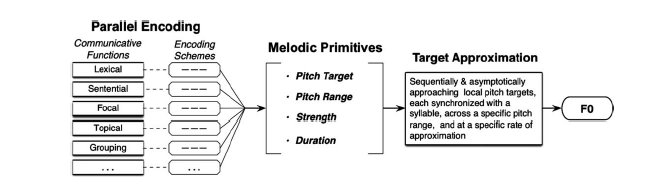
\includegraphics[height=1.5in]{Figures/penta.png}
		\caption{The Penta model: Parallel encoding of different functions in the speech signal \citep[from][]{xu05}}
	\end{center}
	\label{figPenta}
\end{figure*}


A very different conception of how these factors combine to shape the overall prosody of an utterance is assumed in most phonological models of sentence prosody \citep[e.g.][]{pierr80,ladd80,selki84}, and embodied in the ToBI transcription of North American English \citep{beckm97,beckm05}. These accounts are often referred to as the Autosegmental-Metrical Model of sentence prosody  \citep[`AM-Model', cf.][]{ladd08}. They are based on a metrical representation that aligns with the segments of an utterance but is principle independent of it. While in overlay models, the functional dimensions, for example syntactic constituent structure, directly influence the output signal, they do so only indirectly in AM-models. The metrical representation is assumed to consist of a hierarchy of phonological constituents. An example of such a  prosodic hierarchy from  \citet[384]{selki86} is given in Fig. \ref{phi} (we added the Greek letters that are often used to refer to each level, see \citealt{fery13}). Note that the `phonological phrase' is often called `intermediate phrase' instead, e.g. in the ToBI model of American English.


\begin{figure*}[!ht]
	\begin{center}
\setlength{\tabcolsep}{0in}
{\footnotesize
\begin{tabular}{cccccccccccccccl}
\\
\multicolumn{14}{c}{(\_\_\_\_\_\_\_\_\_\_\_\_\_\_\_\_\_\_\_\_\_\_\_\_\_\_\_\_\_\_\_\_\_\_\_\_\_\_\_\_\_\_\_\_\_\_\_\_\_\_\_\_\_\_\_\_\_)}&\hspace{1em}&Phonological Utterance\\
\multicolumn{9}{c}{(\_\_\_\_\_\_\_\_\_\_\_\_\_\_\_\_\_\_\_\_\_\_\_\_\_\_\_\_\_\_\_\_\_\_\_\_)}&\multicolumn{5}{c}{(\_\_\_\_\_\_\_\_\_\_\_\_\_\_\_\_\_\_\_)}&\hspace{1em}{ }&Intonational Phrase ($\iota$)\\
\multicolumn{3}{c}{(\_\_\_\_\_\_\_\_\_\_)}&\multicolumn{6}{c}{(\_\_\_\_\_\_\_\_\_\_\_\_\_\_\_\_\_\_\_\_\_\_\_\_)}&\multicolumn{5}{c}{(\_\_\_\_\_\_\_\_\_\_\_\_\_\_\_\_\_\_\_)}&\hspace{1em}&Phonological Phrase ($\phi$))\\
\multicolumn{3}{c}{(\_\_\_\_\_\_\_\_\_\_)}&\multicolumn{2}{c}{(\_\_\_\_\_\_\_)}&\multicolumn{4}{c}{(\_\_\_\_\_\_\_\_\_\_\_\_\_\_)}&\multicolumn{3}{c}{(\_\_\_\_\_\_\_\_\_\_\_)}&\multicolumn{2}{c}{(\_\_\_\_\_\_)}&\hspace{1em}&Prosodic Word ($\omega$)\\
(\_\_)&\multicolumn{2}{c}{(\_\_\_\_\_\_)}&\multicolumn{2}{c}{(\_\_\_\_\_\_)}&(\_\_)&\multicolumn{3}{c}{(\_\_\_\_\_\_\_\_\_\_)}&\multicolumn{2}{c}{(\_\_\_\_\_\_\_)}&(\_\_)&\multicolumn{2}{c}{(\_\_\_\_\_\_)}&\hspace{1em}&Foot ($\Sigma$)\\
(\_\_)&(\_\_)&(\_\_)&(\_\_)&(\_\_)&(\_\_)&(\_\_)&(\_\_)&(\_\_)&(\_\_)&(\_\_)&(\_\_)&(\_\_)&(\_\_)&\hspace{1em}&Syllable ($\sigma$)\\
\end{tabular}}
\ \\
\caption{The Prosodic Hierarchy according to \citet[384]{selki86}}
\label{phi}
\end{center}
\end{figure*}

In this model, various factors influence the precise prosodic structure. The effect of syntactic constituent structure, for example, may affect the location of phonological and intonational phrase boundaries. Existing phonological models of sentence prosody implicitly or explicitly `build in' specific assumptions about interactions between the different factors influencing sentence prosody. For example, focus is often assumed to influence not just prominence, but also phrasing. The idea is that post-focal material remains unaccented and is `dephrased' (a term from \citealt{jun00}), meaning that it becomes part of the intonational phrase along with the preceding focused material. 

This idea was already implicit in the model of English intonation proposed in \citet{pierr80}. For example, \citet[265]{pierr80} observes that the question in \ref{mani}, with neutral focus, often contains an intonational break between the subject and the VP, as indicated by the percent sign in the example. This break effectively signals that the material within the VP forms a constituent to the exclusion of the subject. This boundary seems to vanish, however, when prominence is shifted to the subject, as in \ref{manifo}, where the entire question is mapped to a single intonational and intermediate phrase. The rise for the intonational phrase boundary is realized at the end, and the rise for the intermediate phrase boundary starts right after the low pitch on {\em Manitowoc}. This rendition of the question with main prominence on {\em Manitowoc} would be adequate as a way to challenge someone else's contextually salient claim that {\em Every small town has a library}: 

\ex. 
\a. Does {\em Manitowoc} \% have a {\em library}?\label{mani}
\b. Does {\em Manitowoc}  have a library?\label{manifo}

The reason behind the assumption that phrasing in the post-focal domain must be erased is that certain categories of phrases (such as intonational or intermediate phrases) are assunmed to necessarily require tonal events----which, the assumption is, cannot be realized post-focally. In general, it should not be possible then to realize phrasing distinctions within the VP of focus is placed on the subject, since the tonal events that cue these phrasing distinctions are not available in an unaccented stretch. The assumption that phrasing is necessarily cued by tonal events is fairly standard in the AM literature. \citet{beckm96}, for example,  argues that ``[\ldots] there must be at least one pitch accent somewhere in every (prosodic) phrase [\ldots]''. Hence in the post-focal domain, where pitch accents are typically absent, phrasing distinctions should be neutralized. 

The question of whether and how focus-induced prominence effects interact with the prosodic phrasing remains central in deciding between current theories of sentence prosody, and is the central research question of this paper. In an earlier test of the claim that early focus obliterates later phrasing distinctions,  \citet{norcl05} found that durational cues for phrasing in the post-focal part of sentences remain intact.  More empirical evidence against (complete) post-focal dephrasing in a variety of languages can be found in \citet{hayes91}, \citet{jun00}, \citet{sugah03}, \citet{ishih03}, \citet{ishih07}, \citet{fery10}, \citet{jun11}, \citet{ishih16} and \citet{kugle17}.  If true, these results speak in favor of an overlay approach, or else of phonological models that do not conflate focal prominence and phrasing. More generally, how various functional dimensions interact can decide between different models of sentence prosody. 

In the following section, we report on prior findings regarding the prosodic realization of the different functional dimensions (speech act, focus, constituency). In section \ref{experiment}, we report on a production experiment with a factorial design that crosses the three functional dimensions  in order to see how they interact in their prosodic effects. Section \ref{forest} will describe an additional analysis using an automatic classification with random forests, which will contribute further insights into the data. We conclude with a discussion of the theoretical implications of our findings for the phonological representation of sentence prosody.


\section{Three Dimensions}
\label{reviewsection}

Focus, syntactic constituent structure, and type of speech act each affect sentence prosody in systematic ways \citep[][]{ladd08}. In this section we will review how the three functional dimensions affect prosodic prominence, prosodic phrasing, and choice of intonational tune, and also point to some potential interactions.


\subsection{Focus and Prosodic Prominence}

In English and many other languages, the prosody of an utterance can be affected by whether a sub-constituent is marked as contextually contrastive or as contextually given \citep[see][for a review of these notions]{krifk08}. 

\ex.\label{water}  
\a.[A:] Jane dove into the water. 
\b.[B:] \# Then Dillon dove into the water.
\c.[B$^\prime$:] Then {\em Dillon} dove into the water.

In A's initial assertion, both the words {\em Jane} and {\em water} typically would carry a pitch accent. In the response to A, however, the VP cannot include a clear and salient accent on water, and prominence has to shift to the subject {\em Dillon}, as in B$^\prime$'s response. How can we explain this? 

Could we simply say  {\em Dillon} receives a contrastive accent in \ref{water} because it contrasts with {\em Jane}, and that this somehow obliterates accents later in the utterance? This characterization would not be sufficient. In the following exchange, there would be no focus prosody in B's utterance, although the two noun phrases, {\em Jane} and {\em Dillon},  contrast here as well: 

\ex.
\a.[A:] Jane sat down. 
\b.[B:] \# Then {\em Dillon} dove into the water.
\c.[B$^\prime$] Then {\em Dillon} dove into the water.

It seems the difference to the prior dialogue is {\em dove into the water} is not previously mentioned here. Could we say instead then that for the prominence shift to obtain, {\em dove into the water} has to be contextually given? This also seems insufficient:

\ex.  
\a.[A:] Dillon dove into the water?
\b.[B:] {\em Dillon} dove into the water.
\c.[B$^\prime$] \# {\em Dillon} dove into the water.

While repeating the whole sentence may not be the preferred way to convey a positive response here, it is certainly a possible one. But using the pronunciation with focus prominence on {\em Dillon} and a reduced VP is impossible---unless B wants to evoke a contrast to somebody other than {\em Dillon} who did or did not jump into the water. The fact that we infer that such a contrast must have been intended is evidence that focus prominence in fact requires a contrast to {\em Dillon}. The correct generalization is that this prosody requires a contrasting alternative of the form {\em x dove into the water}. 

In order to state the correct generalization about focus prosody, we need to refer both to what's contrastive (the material that is substituted in the antecedent), and to what's given (the material that is already present in the antecedent). And both contrastive and given material is acoustically affected by focus: Contrastive material is prosodically boosted, given material prosodically reduced \citep[][i.a.]{eady86,breenetal10}.\footnote{While the arguments given here are hardly sufficient to show this conclusively, see \citet{klassenwagner17} for a series of experiments that support the conclusion that prominence shifts necessarily require contrastive alternatives.} 

\citet{rooth85,rooth92b}, building on ideas in \citet{choms71} and \citet{jacke72}, proposed an influential theory of how to account for focus and givenness effects. At the heart of this account is the notion that each constituent, in addition to its semantic denotation, comes with a set of alternative meanings (in the trivial case, just the meaning of the constituent itself).
A second ingredient of this theory is the syntactic operator $\sim$, which can attach to any constituent and operates over its alternatives. It introduces the presupposition that a set of alternatives to this constituent is contextually salient. The antecedent alternatives have to be identical to the constituent $\sim$ attaches to, modulo substitutions of constituents that bear a syntactic F-marker. In this theory, B's response in \ref{water} would be represented as follows:

\ex. Then [[{\em Dillon}]$_F$ dove into the water]$\sim$\label{waterFoc}

According to this theory, the utterance in \ref{water} requires a contextually salient set of semantic alternatives of the form  {\em x dove into the water}, where $x$ stands in for one or more contextually relevant alternatives to {\em Dillon}. One can characterize the prosodic effect of $\sim$ as follows: F-marked material within the scope of $\sim$ (`material marked as focused') is prosodically boosted, while non-F-marked material in the scope of $\sim$ (`material marked as given') is prosodically reduced  (cf. \citealt{rooth92b,truck95}). This can be thought of a constraint on  the relative prosodic prominence between constituents: Focused constituents need to be more prominent than given constituents \citep[cf.][]{willi97,  szend03, wagner05recursion, reinh06, burin16b}. The focus presupposition in \ref{water}, for example, is encoded by flipping the relative prominence relation between subject and VP. Whereas by default, the VP must be more prominent than the subject, the focus structure in \ref{water} has the effect that the subject must be more prominent than the VP. 

This notion of `relative prominence' is of course not an innocent assumption. An important question for prominence-based approaches to focus-marking is whether the notion of relative prominence is directly entwined with the notion of prosodic phrasing, which also affects perceptual prominence. Our data will provide new insights on this question, which will discuss in detail the final section of the paper. %For example, in the prosodic hierarchy the assumption is that the heads of higher level prosodic phrases (such as intonational phrases) are more prominent that than the heads of lower-level prosodic phrases that are  (such as the case of a prosodic word that is not itself the head of an intonational phrase). In this kind of approach, placing focus on a particular word requires making it the head of an intonational phrase and preventing non-focused words to also receive equal prominence, and thus requires post-focal reduced material to be part of the same intonational phrase. %Another possibility, however, is that prominence is represented independently of phrasing, as  is assumed in the metrical representation in \citet{wagner05recursion}, or that at least phonological phrasing is maintained in the post-focal domain. This requires flexibility within intonational phrases with respect to which particular head of a phonological becomes the head of the intonational phrase \citep[as is assumed in ][]{burin10typology, fery13, burin16}. 
\footnote{There are different accounts of how the phonological reflexes of focus marking that do not require a notion of relative prominence.  \citet{schwa99}, for example, argues that all and only F-marked words carry a pitch accent. The assumption fails to explain asymmetries between the last (or `nuclear') accent of an utterance and prior accents. \citet{welby03} found that the presence of prenuclear accents do not come with the interpretive effects of focus, while the presence of the nuclear accent does. These asymmetries make sense if relative prominence is what's crucial, and if, other things being equal, final constituents are more prominent than earlier constituents. We return to this below. Another weakness this account is that it fails to explain how focus can still be encoded in the absence of any pitch accents, such as in instances of second-occurrence focus \citep{burin16b,bauma16}.}

Prior studies have shown that the  phonetic realization of focus prominence in English involves an increase in duration, pitch range, and intensity of the stressed syllable of the focused constituent, and a reduction in duration, pitch range, and intensity on the material following the focused constituent \citep[][i.a.]{coope85, eady86, breenetal10}. The pitch range reduction has been reported to manifest itself differently depending on the intonational tune of an utterance. In a declarative utterance, pitch usually drops right after the accented syllable of the focused constituent and remains low throughout the post-focal domain. In an utterance with a rising question intonation, pitch usually rises right after the focused constituent and remains high throughout the entire post-focal domain. 

The phonological interpretation of this post-focal reduction varies in the literature. While prior analyses often assume that post-focal constituents are completely deaccented and without any tonal targets, there are several reports of pitch movements in the post-nuclear domain, starting with \citet[223]{pierr80}, who observed post-nuclear `echo accents.' Findings of this type  have lead some authors to posit that post-focal reduction does not obliterate pitch targets altogether, but rather, it may simply compress pitch events to a more narrow range \citep[e.g.][]{sugah03, ishih03, ishih16, kugle17}.  Another interpretation of at least some post-nuclear tonal events are that they are the reflex of (intermediate) phrase-accents, and align with metrically prominent syllables \citep[see][for a detailed discussion of phrase accents]{grice00}.

Our main research question here is how focus prominence affects prosodic phrasing, and more specifically whether the cues to phrasing are obliterated, or at least diminished, in the post-focal domain. In order to better understand why such an effect might be expected, let's look at how prosodic phrasing is assumed to come about. 


\subsection{Syntactic constituent Structure and Phrasing}

Syntactic constituent structure affects the durational pattern of utterances, such that prosodic domains (such as the phonological phrase or the intonational phrase) often comprise words that form syntactic constituents and exclude words that are not part of the constituent. Hence, prosodic phrasing often encodes syntactic constituent structure. \citet{lehis73} demonstrated this convincingly in a study looking at whether globally ambiguous sentences are acoustically differentiated when said aloud. While some structural ambiguities were not reliably disambiguated (e.g., PP attachment ambiguities), others were. An example are coordinate structures:

\ex.\label{2lehis}
\a. (Steve or \underline{Sam) and Bob} will come.\label{2lehisa}
\b.  Steve or \underline{(Sam and Bob)} will come.\label{2lehisb}

\noindent One central finding was that the length of the underlined parts of these coordinate structures were longer if they contained a syntactic constituent boundary (marked with a parenthesis here).  There are multiple durational lengthening effects that contribute to these differences. \citet{klatt75} found that syllables that occur at the end of syntactic constituents are substantially lengthened.  Many studies since have supported the presence of domain-final (or pre-boundary) lengthening in English and other languages \citep{wight92, price91,shatt96,byrd98,cho01,byrd03,cho16}. In the coordinate structure in \ref{2lehisa}, {\em Sam} would be longer compared to the strucure in \ref{2lehisb} because it occurs at the end of a larger syntactic unit. \citet{turk07} found the boundary-induced lengthening affects both the final syllable before the boundary as well as the last accented syllable preceding it. 

 \citet{wagner05recursion} investigated durational effects in coordinate structures in more detail, and found that there is also a speed-up in words that occur at the beginning of a phrase, compared to the durations observed in a simple list structure without internal syntactic branching. A second finding of interest was that the degree of pre-boundary lengthening induced by syntactic junctures within an utterance is often much greater than the final lengthening observed at the end of an utterance. In coordinate structures similar to \ref{2lehis},  the durational difference in the final words in coordinate structure (in our example the name {\em Bob}) did not show a big variation depending on its position in the structure, and generally showed a duration more comparable to utterance-internal words that were not phrase-final. 
 
The distribution of pauses provides a further cue to syntactic grouping. Pauses have been reported as correlating less well with syntax than duration \citep{gollr13}, probably because they can also be due to other cognitive factors, such as lexical retrieval or other types of processing difficulty \citep{goldm72}. \citet{grosj79} conducted an experiment in which participants read sentences at different speech rates. They added the average pause-length between each set of two adjacent words. They could then derive a hierarchical tree structure of these sentences based on the phonetic closeness of pairs of adjacent words. These trees  closely matched participants' intuition about how they would group these words.  \citet{gee83} propose a prosodic interpretation of these effects, such that the length of a pause between two words can be a cue to whether and to what extent they phrase together prosodically. Within the ToBI system of intonation, pauses are viewed as evidence as to whether there is an intonational phrase break (high likelihood of a pause) or an intermediate phrase break (lower but non-zero chance of a pause). It also includes a category (break-index 2) which is used when either a pause is present but a tonal boundary signal is absent, or when a tonal boundary signal is present but the disjuncture sounds `weaker than expected' for an intermediate or intonational phrase break \citep[35]{beckm97} . There is some evidence that pre-boundary lengthening and pauses are perceptually integrated into a single percept of juncture. \citet{Marti70, Marti71} found that listeners report hearing pauses although there were no unfilled pauses in the signal when there was syllable lengthening just before the perceived juncture. 

Apart from final (or pre-boundary) lengthening and pause placement, phrasing has additional durational effects due to domain-initial strengthening  \citep{fouge97, lavoi01, cho02, keati03,keati06,cho07,cho11,cho16}. Domain-initial strengthening occurs at the beginning of prosodic domains, and the degree of strengthening increases cumulatively with the strength of the prosodic boundary.  \citet{fouge97} investigated initial strengthening in arithmetic expressions:

\ex. (89 + 89 + 89) * 89 = a lot. \label{2arithm}

\noindent Participants were recorded using so-called `reiterant speech, which  mimics the structure of such arithmetic expressions:

\ex.(nonono no nonono no nonono) no nonono equals a lot

\noindent The results showed that nasal onsets were realized with more linguo-palatal contact at the beginning of larger prosodic phrases, which also resulted in a longer duration of these nasals. Similar results were reported from an acoustic study of VOT in Korean in \citet{Jun93}.  \citet{keati03} reviews cross-linguistic evidence showing that such initial strengthening effects are pervasive.

Apart from duration, there are also F$_0$ cues to phrasing. The most important reason why F$_0$ often provides cues to phrasing are boundary tones \citep[][i.a.]{pierr80,ladd08}. Interestingly, \citet{gollr13} found in a series of production and perception experiments that F$_0$ related cues to boundaries are important when conveying intonational phrasing, but less important when conveying (smaller) phonological phrase boundaries. 

Apart from affecting boundary-tone placement, prosodic phrasing has also been reported to affect the relative scaling of pitch accents \citep{ladd88}. These scaling effects are  often attributed to an adjustment of a reference line for pitch that is sensitive to prosodic phrasing. The idea is that individual tonal targets are scaled relative to this reference line. \citet{ladd88} coordinated sentences as a way to probe for pitch scaling effects and found clear scaling effects between intonational phrases:

\ex.\label{laddoo}
\a. Ryan has a lot more money, (but Warren is a stronger campaigner and Allen has more popular policies).\label{laddoa}
\b. (Ryan has a lot more money and Warren is a stronger campaigner), but Allen has more popular policies.\label{laddob}

\noindent In structures of the type in Example \ref{laddoa},  the pitch level on the last conjunct ({\em Allen has more popular policies}) is down-steppped relative to the conjunct that precedes it ({\em Warren is a stronger campaigner}), which in turn is down-stepped relative to the first ({\em Ryan has a lot more money}). In Example  \ref{laddob}, on the other hand, the pitch-level in both the second and third conjunct are down-stepped relative to the first. Ladd takes these scaling differences to motivate  a hierarchically organized metrical representation with recursively nested intonational phrases.  \citet{vanden92} show similar  scaling effects in coordinate structures involving place names. More evidence for pitch scaling is discussed in \citet{Kuboz89}, \citet{Kuboz92}, \citet{vanden92}, \citet{fery05},\citet{fery10b},\citet{kentn13},\citet{truck15}, and \citet{petro17}.

%There have been varying accounts of F$_0$ scaling in terms of such a reference pitch or register level \citep{ladd88,vanden92,fery05,fery10b,kentn13,truck15,petro17}.

Intensity is often not considered as a cue to phrasing. For example  \citet{price91} and \citet{wight92} explore pitch and durational cues, but make no reference to intensity. \citet{stree78} considered amplitude as a cue for boundary perception, but concluded it is only of minor importance. 

One reason why intensity is often disregarded may be is that existing correlations between phrasing and intensity could be chalked up as an automatic consequence of exhalation, rather than an actively controlled cue. A drop in intensity over the course of an utterance is expected because exhaling reduces sub-glottal pressure \citep{bjork16}. There are indeed many reports that intensity tends to decrease throughout an utterance. \citet{pierr79} reports experimental evidence for such a down-drift, and also that it interacts with the perception of prominence in perception: Failing to decrease intensity on later constituents provides a cue for prominence.  

There is some indication, however, that speakers might actively control intensity in order to cue prosodic phrasing. \citet{trouv98} provides an example of how intensity can be used as a cue for a phrase break in English. In a production study on prosodic phrasing in German, \citet{poschmannwagner16} found that intensity is a cue to phrasing comparable in reliability to pre-boundary lengthening, such that intensity is adjusted high at the beginnings of phrases and then drops toward the end of the phrase. This was found to be a cue for phrasing distinctions even utterance-medially, so the scaling of intensity did not appear to be simply a result of the drop in sub-glottal pressure while exhaling.  

One important aspect of intensity in speech is that it closely correlates with pitch. For example, speakers raise F$_0$ when aiming to talk louder for about a half semi-tone per db \citep{gramm88}. See also the discussion in \citet{vaiss83}. But this is not a physical necessity, speakers can in principle also talk louder while holding pitch constant. The heightened air-flow may just naturally increase the frequency of vocal fold vibration unless a speaker counter-acts that tendency. This raises the possibility that some variability of pitch due to phrasing (such as pitch-accent scaling) may actually be a passive consequence of an active manipulation of intensity by the speaker, or may just be used to enhance the primary cue of intensity. Our results will support the conclusion that intensity is an excellent cue to phrasing in English, and in fact a much better cue than pitch.



\subsection{Speech act and Intonational Tune}

Intonational tunes vary depending on the speech act that an utterance performs. The choice of intonational tune is typically assumed to affect only the tonal events of an utterance. For the present study, only declarative falls and the rises frequently used in polar questions are relevant. One distinguishing feature between these two tunes is that they end in different boundary tones, an L\% in the case of the declarative fall and an H\% in the case of interrogative rises. The interrogative rise is typically used in polar questions, it can also be used in wh-questions \citep{hedbe14}; the declarative fall is typically used in declarative assertions and wh-questions, but sometimes also in polar questions. The semantic differences between these tunes remains an open research question \citep[see][for a review]{truck12}. 

The final rise in polar questions and the final fall in declaratives often seems to start right after the pitch-accented syllable, rather than at the end of a phrase or the utterance. This is often attributed to there being `phrase accents' in addition to the final boundary tones as part of these tunes, following \citep{pierr80}. These are today usually taken to be boundary tones of intermediate phrases, even though they are realized right after the pitch-accented syllable \citep[see][for a review and empirical evidence in favor of phrase accents]{grice00}. 

Finally, the two tunes also differ in the pitch accents that are placed on accents words within an utterance. The English question rise is usually used with L* pitch accents, while the English declaratives fall usually with H* or H*L pitch accents, although other combinations are possible \citep{pierr90}. Duration and intensity may also be cues to differentiate different intonational tunes, but they are often not considered---our results will show they, too, can distinguish different contours. 


\subsection{Interactions}

The central research question of this paper is how cues to focus prominence and cues to prosodic phrasing interact. More specifically, we are interested in the question of whether prosodic phrasing remains intact in the post-focal domain.  There is some prior work that suggests that at least durational cues remain intact \citep{norcl05} in English \citep[see][for relevant results in other languages]{jun00, sugah03, ishih03, ishih16, kugle17}.  The question of whether pitch cues to phrasing are used in the post-focal domain is still unresolved, although  there are studies that suggest that the often-made claim that there are no tonal targets in the post-focal domain might not be accurate at least in some languages \citep{xu05,  kugle17}. It is possible that  post-nuclear tonal perturbations are due to phrase accents that do not constitute full pitch accents---we will return to this issue in the final discussion.

While prosodic phrasing, just as focus prominence, affects duration, intensity, and F$_0$, among other things, their precise effects differ phonetically in where exactly in the signal they occur \citep{edwar91, beckm92b, cho09, cho11}. For example, phrase-final lengthening mostly affects the final syllable, while lengthening due to prominence mostly affects the accented syllable. And yet the effects of accentual lengthening spill over into following unstressed syllables \citep{turk97} and final lengthening can also affect the accented syllable \citep{turk07}. There are also good reasons to think that prosodic phrasing might be affected by focus more directly. In many languages, focus appears to affect phrasing decisions \citep[][and references therein]{fery13}. Conversely, phrasing also seems to affect our percept of prominence. In Lehiste's coordination examples in \ref{2lehis}, {\em Sam} seems intuitively more prominent when at the end of a prosodic phrase as in (a) than at the beginning, as in (b). Various models have claimed that this is {\em why} focus affects phrasing: foci like to align with the edges of prosodic phrases because it makes them more prominent \citep{truck99,burin10typology}, which fits well with the Roothian prominence-based approach to focus \citep[but see][for a different perspective]{fery13}.  

We are also interested in other types of interactions. The choice of intonational tune, which is affected by the type of speech act, might also interact with how focus and phrasing are encoded. For example, utterances with question rises might have very different pitch accent scaling effects.  The question whether and how pitch-accent scaling is used in questions has also not been previously explored, as far as we know, although there is work on the realization of prosodic boundaries in questions as opposed to declaratives. A reviewer pointed us to \citet{feldh16}, who found that in Spanish, while dislocated topics typically end with a rise in declaratives, in questions they often end with a fall and are obligatorily followed by a pause.  According to Rooth's theory of focus, the choice of intonational tune should in principle be orthogonal to the prosodic effects of focus. But recently, such interactions have been found:  \citep{goodhueetal16} found that focus prominence is almost never used when the Contradiction Contour is chosen, but in the same context is used very frequently when a declarative fall is used. \citet{schlo18} argues that focus prominence is used differently with the rise-fall-rise contour. 

Finally, while the role of intensity is often considered in studies of focus prominence, its role in cueing phrasing or intonation has not been given much consideration in the literature. While many prior studies have looked at the role of intensity as a cue for prosodic prominence, we are not aware of work that looks at how this interacts with the choice of tune or phrasing. 

Having reviewed some key findings about cues to all three dimensions, and some particular claims about interactions between them, we can now turn to our experiment. The study crosses all three functional dimensions and aims at establishing how independently or interactively they affect the output prosody.


\section{The Experiment}
\label{experiment}

By crossing the three functional dimensions  (speech act, focus, constituent structure), we will be able to test their individual phonetic import on the signal as well as whether they interact with each other. Prior studies have usually only manipulated one dimension at a time, or at most two.  \citet{eady86}, in their classic study on sentence prosody, looked at focus and type of speech act (question vs. declarative), for example. We are interested here in whether the contribution of all three functional dimensions can be successfully retrieved from the acoustics, or whether the effect one sometimes neutralizes the effects of the other. Of special interest is the question of whether acoustic cues to phrasing remain intact in the post-focal domain. 

\subsection{Methods}

\subsection{Speech materials}

For our manipulation of constituent structure, we used coordinated names \citep[following][]{lehis73, vanden92, wagner05recursion, fery10b,kentn13,petro17}. The intended syntactic constituent structure was indicated by the placement of commas.  \ref{left} illustrates an example with left-branching ([AB]C), and \ref{right} illustrates right-branching (A[BC]):\footnote{See the supplementary materials for a complete list of the stimuli.}

\ex. Declarative, Focus on Conjunct B, Left-Branching:\\
 {\footnotesize You said that Megan and Dillon, or Morgan would help. But in fact we were told that Megan$_A$ and Lauren$_B$, or Morgan$_C$ would help.}\label{left}
 
\ex. Declarative,  Focus on Conjunct B, Right-Branching\\
 {\footnotesize You said that Megan, and Dillon or Morgan would help. But in fact we were told that Megan$_A$, and Lauren$_B$ or Morgan$_C$ would help.}\label{right}
 
We varied the type of speech act simply by using a period at the end of the target utterance as in \ref{left} and \ref{right}, indicating that it was intended as an assertion, or alternatively a question mark \ref{ques}, indicating that it was intended as a polar question. We expected that participants would produce a rising intonation for questions, since this is the canonical intonation for polar questions in American English \citep{ladd08, hedberg2010prosody}.\footnote{\citet{eady86}, who also were interested in focus realization in rising question tunes, looked at declaratives vs. wh-questions instead. This seems like a risky choice, however. Most polar questions in American English are realized with a rising intonation, and especially those with declarative syntax are very likely to, in order to avoid confusion with a declarative interpretation; wh-questions,m on the other hand, are realized with a falling intonation \citep{hedberg2010prosody}. Nevertheless, \citet{eady86} report that most of their participants produced a rising intonation for they wh-questions---this may have been due to explicit instruction. Our participants were not instructed to use rising intonation for our polar questions, but did so nevertheless, almost always.}

 \ex. Interrogative, Broad Focus, Left-Branching\\
 {\footnotesize You said that Dillon would help. But now it turns out that Megan$_A$ and Lauren$_B$, or Morgan$_C$ would help?}\label{ques}
 
For the manipulation of focus, we varied where there was a contrast in the two clauses that the speakers produced.  For example, in \ref{left} and \ref{right}, the second part of the utterance contrasts with respect to the choice of the second name (focus on $B$, or `second focus'), while \ref{ques} the entire coordinate structure in the second clause contrasts with {\em Dillon} in the first clause, so the entire coordinate structure is focused (`broad focus'). Many papers on prosodic focus marking distinguish different types of focus \citep[e.g.][]{gusse07}. Our declarative examples can best be characterized as `corrective focus' \citep[cf.][]{ladd08, vanderkloketal18}. Our interrogative are similar, in that they involved echo questions, which are closely related to corrective focus in declaratives, in that they also either correct or at least double check a contextually salient antecedent.

Overall, the experiment involved two different types of speech acts (question vs. declarative), four focus conditions (focus on conjunct A, B, or C, or  broad), and two different constituent structures for the coordination (A[BC] vs. [AB]C), for a total of 16 conditions. We had four different item sets varying in these 16 conditions, that differed in lexical content, for a total of 64 different target sentences.


\subsection{Procedure}
%Second, a thorough revision of the methods section is needed, e.g. with more information on the exact instructions given, the recordings, the measurement of the acoustic parameters (explain what was measured and why, e.g. why only word durations, which intensity measure was used, why F0 mean and not the more informative measures F0max/min and/or F0 slope), and the normalization and residualization procedures (as well as the interpretation of the latter). Furthermore, some discussion on the relation between the measured F0 values and pitch accent types (and boundary tones), i.e. to phonological structure in general, would be desirable. Finally, do not mix levels of description, e.g. by equating focus and (prosodic/accentual) prominence!

The experiment was conducted in a sound-attenuated booth at McGill, using a Logitech H390 headset. Speakers were instructed that the study is about speech production, but were not told that we were specifically interested in prosody and intonation. The experiment was conducted using Matlab scripts developed in our lab for running simple production and perception experiments. On the first screen, participants saw instructions about the experiment. They were asked for each trial to  first read the target sentences silently, and to proceed with the recording when they felt ready to be recorded.  They were instructed to `say the sentences as naturally as possible, as if you were saying them to a friend in an everyday conversation.' Each utterance consisted of two parts, a set-up sentence and the target sentence. Participants did not get the option of rerecording if they felt unhappy with their first try.

Every participant was recorded on all 64 sentences. The manipulation of speech act was done between two experimental sessions of 32 trials each, which were separated by a filler experiment. About half of the participants were first run on the questions, and the other half were first run on the declaratives.  In each session, trials were presented in a pseudo-randomized order maximizing repeated trials from the same item set, and only allowing maximally one repetition of the same condition. 


\subsection{Participants}

A total of 25 native speakers of North American English participated (20 female, five male). They were compensated for their participation. They participated in a language questionnaire about their linguistic background. Eight of the participants reported to be fluent in one or more languages other than English, three reported speaking another language natively. We did not consider linguistic background in analyzing our data, but whether speakers were fluent in another language did not seem to have any obvious differences in their results. 


\subsection{Annotation and Quality Control}

The recorded sentences were manually checked for speech errors, disfluencies, hesitations, and recording errors. Only fluent utterances were kept. This step resulted in the exclusion of  24\% of the data, which were more or less evenly distributed across the various conditions.\footnote{We included a table with the number of observations per conditions in the supplementary materials.}  The high exclusion rate is likely due to the length and complexity of the stimuli. Due to additional trials where the recording didn't work (probably because participants pressed the key too early), only 70\% of all trials were used (1,166 utterances out of 26*64=1,664 soundfiles). 

In order to check whether our manipulations were successful, two research assistants annotated the data. They were asked to decide whether the intonation was falling or rising, what the prosodic phrasing of the coordinate structure was, and which of the four focus prominence options was likely intended. For each dimension, they could also choose `unclear' if they were not sure. Inter-annotator agreement was `almost perfect' for the annotation of intonation (Cohen's kappa: 0.96), and `substantial' for constituency (Cohen's kappa: 0.73) and prominence (Cohen's kappa: 0.63). 

Overall, the annotation matched very well with the prosodic realization that was expected given the manipulation for all dimensions. One annotator marked the intonational tune according to expectation (that is, declaratives were annotated as falling, and questions as rising) 96.3\% of the time (chance would be 50\%); the expected bracketing  61\% of the time, with about one third of soundfiles marked as `unclear' (chance would be 50\%); and the expected focus prominence  38\% of the time (chance would be 25\%). The second annotator was slightly less accurate, but showed a similar overall pattern. These results suggest that our manipulation successfully lead to different prosodic realizations for all three dimensions. The accuracy of the focus prominence annotation is not very high, however. There was a high rate of confusion of broad vs. third focus (that is, focus on the C), and 21\% of utterances marked as `unclear.' We will discuss this in more detail in section \ref{forest}. Since we did not want to bias the results based on prior expectations, we included all all of our data in our overall analysis irrespective of whether our annotators were able to correctly annotate them, for a total of 1,166 sound files. 


\subsection{Acoustic Processing of data}

The recordings were aligned with the Montreal Forced Aligner \citep{mcauliffeetal17}, using acoustic models trained on LibriSpeech \citep{librispeech}. The aligned dataset was analyzed with PolyglotDB \citep{polyglotdb}, a software library that can be used for further speech processing. We automatically extracted pitch measures using through Praat's F$_0$ analysis, using 50Hz and 500Hz as the minimum and maxium F$_0$, respectively. Once automatic measures were extracted, each utterance F$_0$ track was hand-checked for octave doubling/halving errors with a software interface developed at McGill.\footnote{To reduce the considerable differences in F$_0$ between speakers and to control for any vowel-intrinsic effects on F$_0$, we considered using a relativized measure of mean F$_0$, calculated  in PolyglotDB.  This relativized measure was a z-score of the F$_0$ using per-speaker means, per-segment means, and standard deviations.  The summary statistics were calculated based on all segments in the corpus, including those in words outside the target words (e.g., the relativized measures would adjust for the intrinsic pitch, duration, and intensity of segments, and also for by-speaker variation due to speech rate, gender, etc.). This normalization, however, did not substantially improve how visible the effects of interest were. In the interest of having easily interpretable measures, we decided to stick to unrelativized measures in this paper. The use of mixed-effects models, the random effect structure can capture these sources of variability to a large extent anyway.}  Intensity was likewise extracted through PolyglotDB, and relied again on Praat's analysis. Duration was calculated with the forced-aligned boundaries.  We decided to use acoustic measures for the first and last syllable of the three target words in the coordinate structure. For each syllable, we extracted the duration, the maximum F$_0$, and the mean intensity. 

To illustrate what the recorded utterances were like, let's consider some examples from one of the speakers.  Fig. \ref{examm} shows two utterances with first focus and a falling declarative intonation, for both types of branching;  Fig. \ref{examm2}  shows two utterances with first focus and rising interrogative intonation, for both types of branching. 

%add textgrid; 
% add declarative versions
\begin{figure*}[ht!]
	\begin{center}
	\parbox{4.25in}{
	        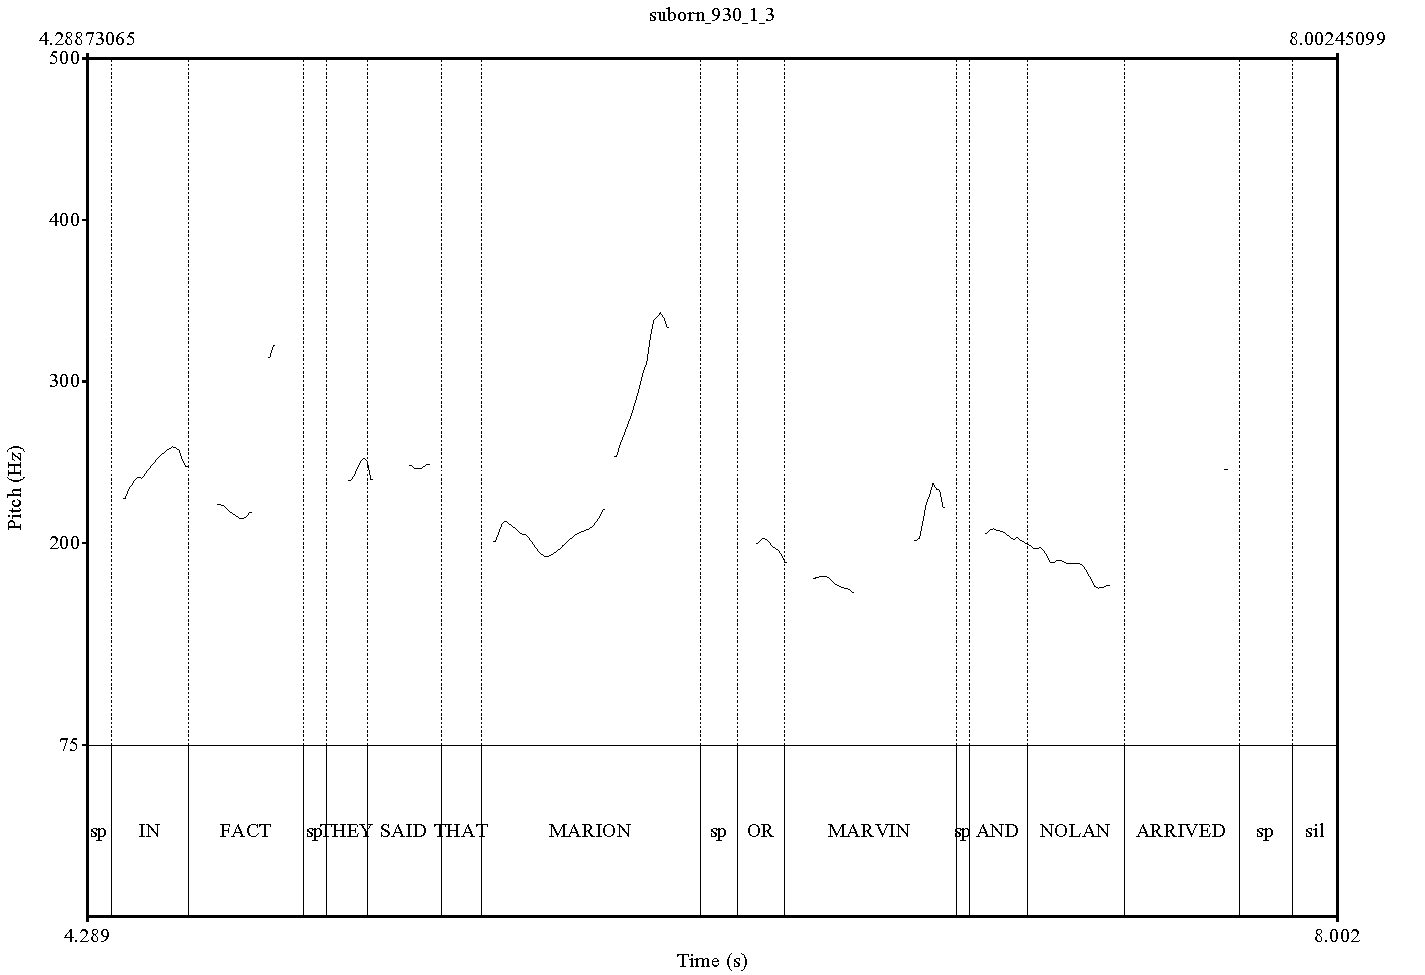
\includegraphics[width=4.25in]{Figures/suborn_930_1_3.pdf}\ \\
	        \href{http://prosodylab.org/~chael/sounds/pape2017/suborn_930_1_3..wav}{\footnotesize\ ... (Marion or Marvin) and Nolan arrived.}
	        }
	        
	        %\parbox{0.05in}{\ }
	        \parbox{4.25in}{
	           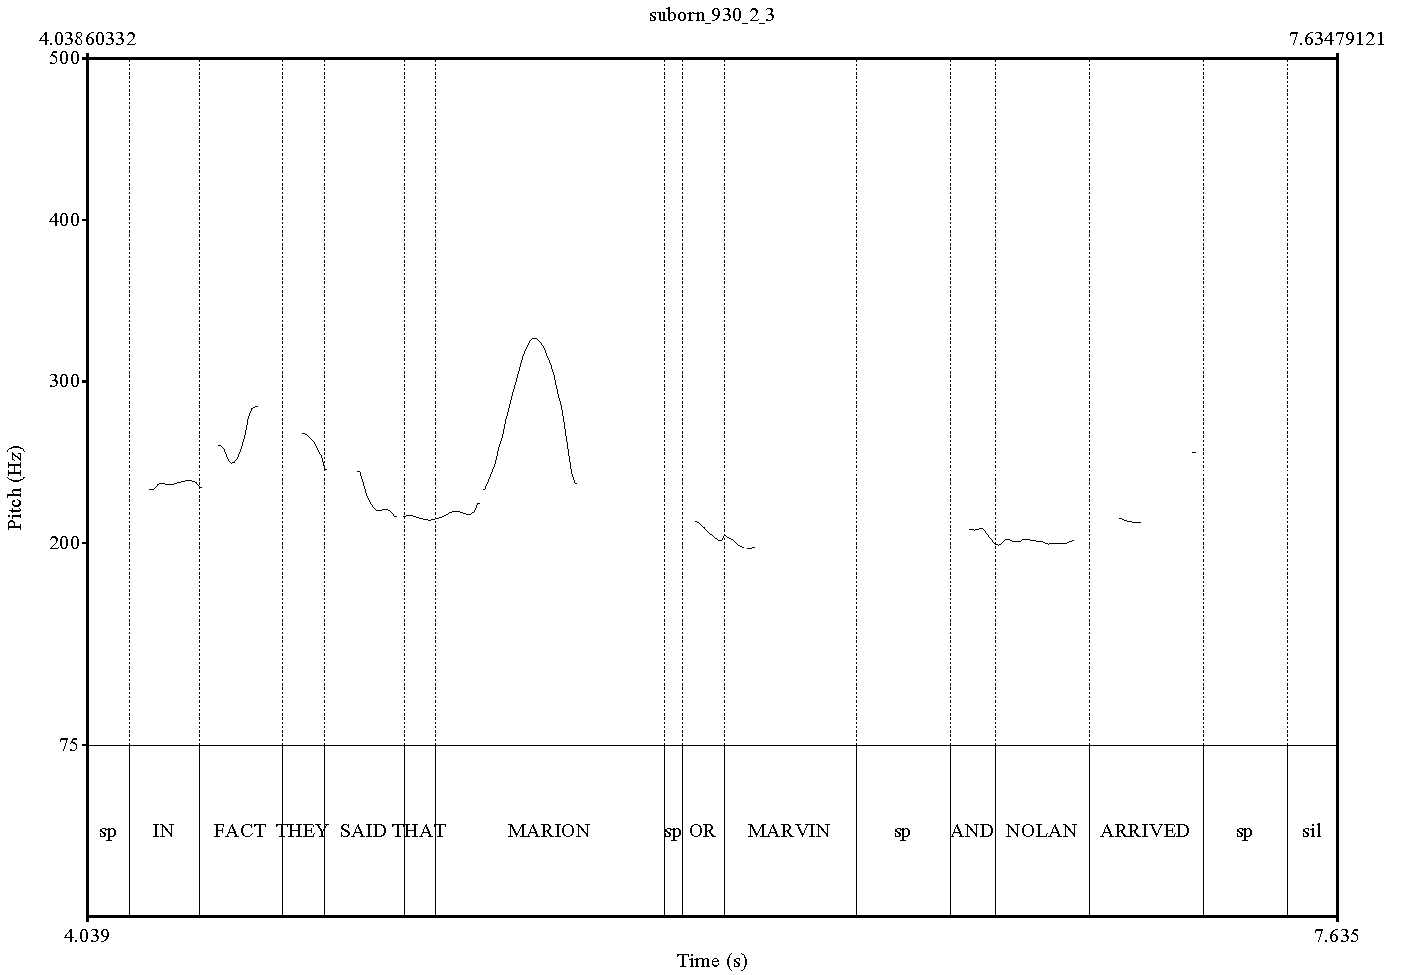
\includegraphics[width=4.25in]{Figures/suborn_930_2_3.pdf}\ \\
	            \href{http://prosodylab.org/~chael/sounds/pape2017/suborn_930_2_3..wav}{\footnotesize \ ... Marion or (Marvin and Nolan) arrived.}
	            }
	            
		\caption{Two examples with initial focus a falling declarative intonation, differing in constituent structure.}
		\label{examm}
	\end{center}
\end{figure*}	            
	         
\begin{figure*}[ht!]
	\begin{center}	            
	            \parbox{4.25in}{
	             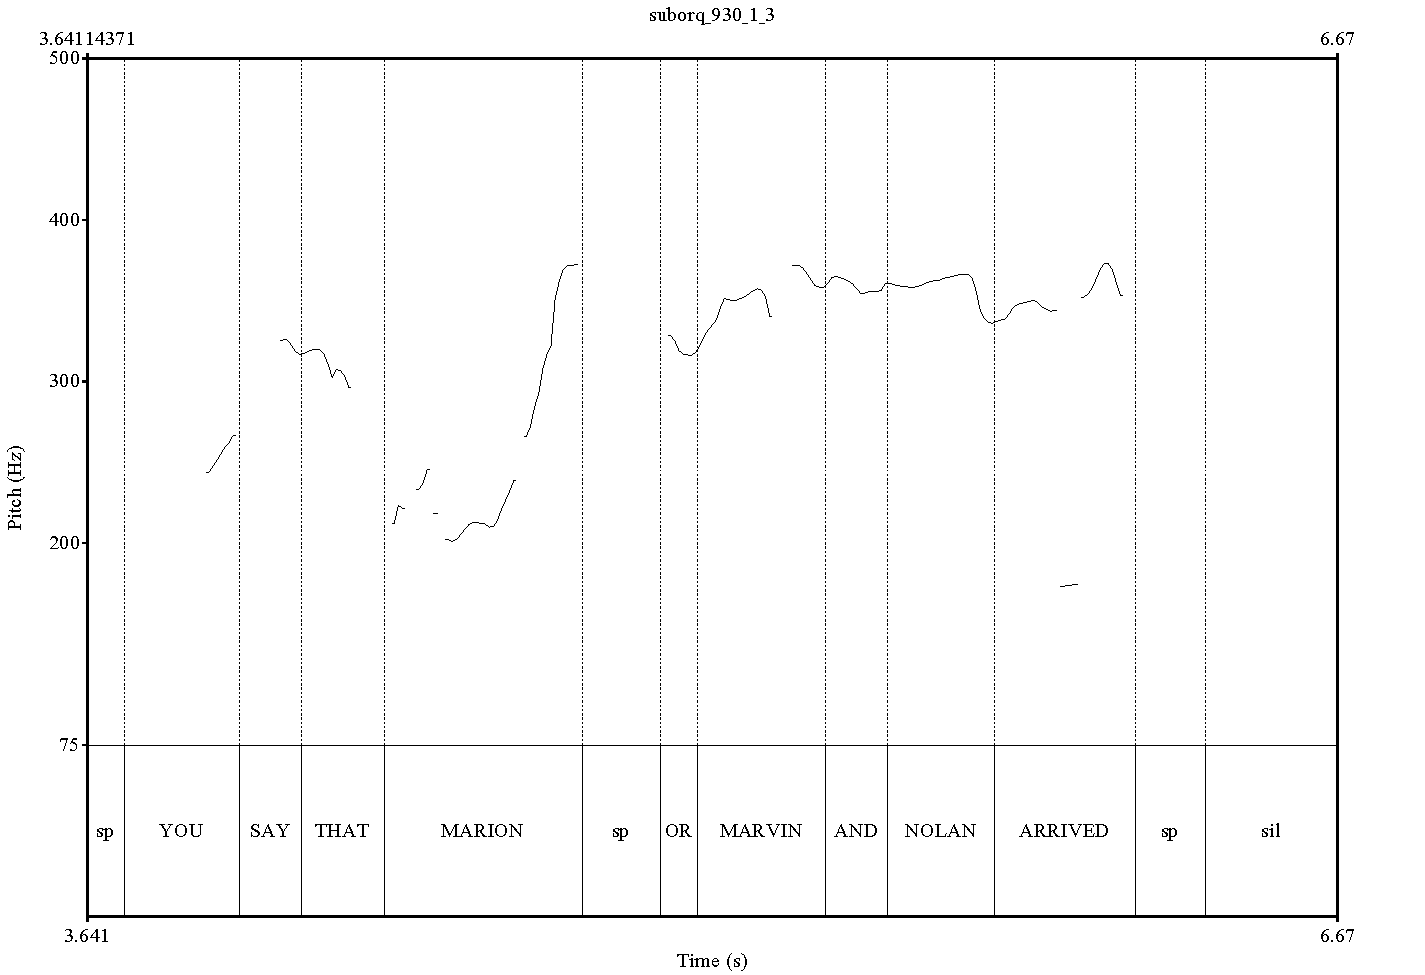
\includegraphics[width=4.25in]{Figures/suborq_930_1_3.pdf}\ \\
	        \href{http://prosodylab.org/~chael/sounds/pape2017/suborq_930_2_1..wav}{\footnotesize\ \ ...(Marion or Marvin) and Nolan arrived?}
	        }
	        
	        %\parbox{0.5in}{\ }
	        \parbox{4.25in}{
	           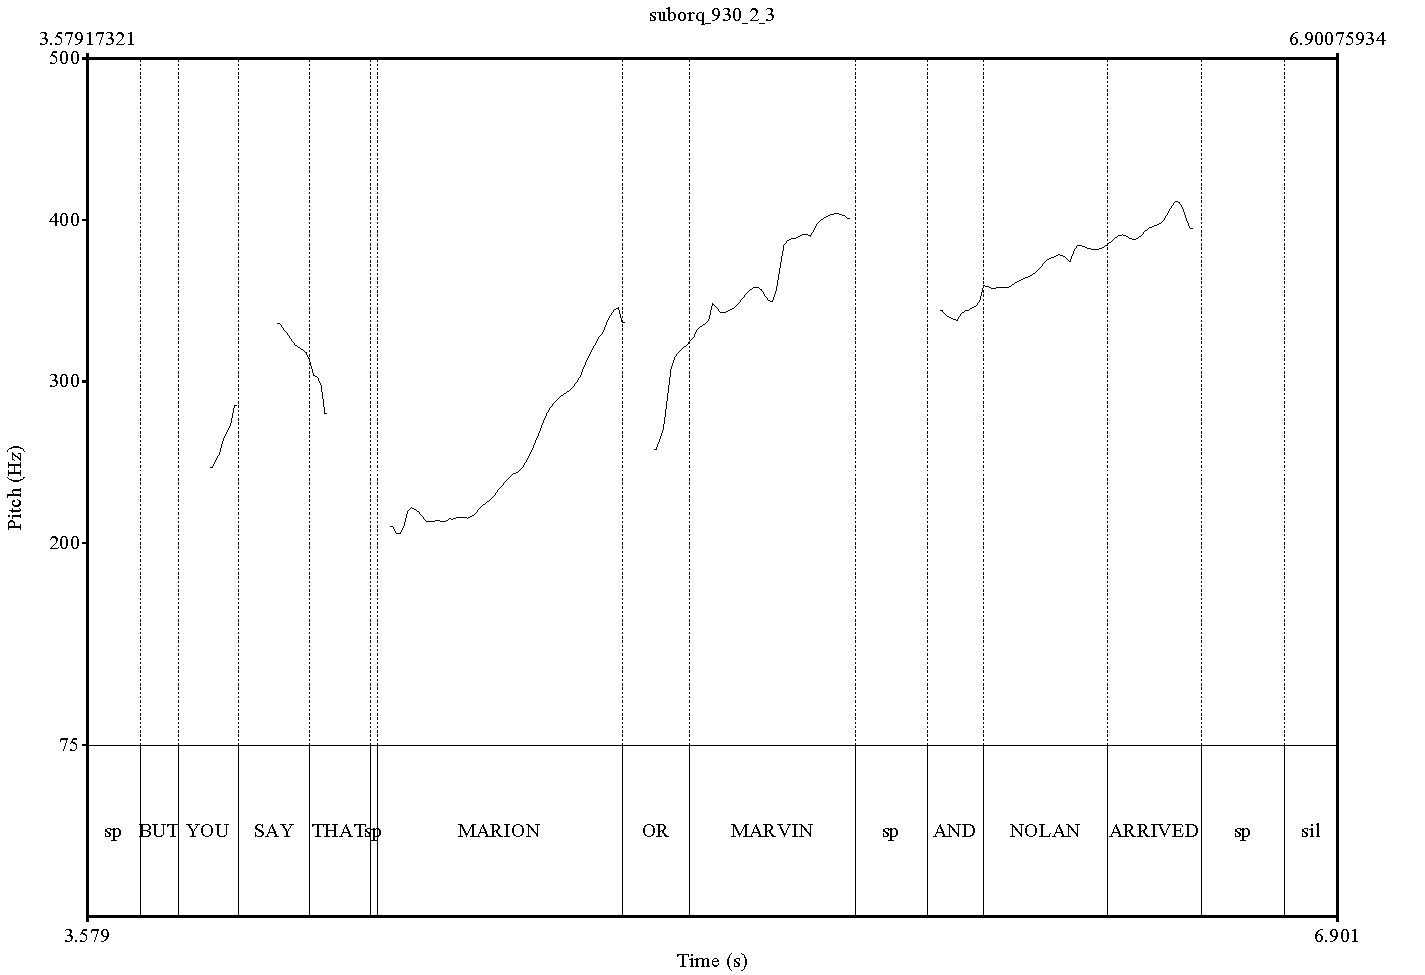
\includegraphics[width=4.25in]{Figures/suborq_930_2_3.pdf}\ \\
	            \href{http://prosodylab.org/~chael/sounds/pape2017/suborq_930_2_3..wav}{\footnotesize\ \ ...Marion or (Marvin and Nolan) arrived?}
	            }

		\caption{Two examples with initial focus and rising question intonation, differing in constituent structure.}
		\label{examm2}
	\end{center}
\end{figure*}	

The utterances clearly convey the post-focal phrasing for both intonational tunes, but they also clearly encode initial focus.\footnote{The coordinate structures below the pitch tracks link to the soundfiles that the reader may want to listen to in order to get an idea what the productions sounded like.} This is visually obvious in the different durations. It is less obvious whether the pitch track carries any independent information about phrasing. In the two utterances with rising question intonation, the focused constituent appears to carry a low pitch accent. The rise of the question involves a final H\% boundary tone. Note, however, that instead of a gradual rise toward the end of the utterance, there is a sharp  rise  immediately after the pitch-accented syllable. This kind of pattern is analyzed in \citet{pierr80} as being due to a `phrase accent'. Similarly, in the utterances with declarative intonation, there is a sharp fall right after the focused constituent. \citet{pierr80} analyzed phrase-accents as being the reflex of intermediate phrase boundaries, even though they often align with prominent syllables within the utterance rather than the edge of the phrase. See \citep{grice00} for more evidence for this analysis. Just based on observable tonal events, it seems then that there are no intermediate or intonational phrase boundaries in the post-focal domain, and yet there are clear clues to post-focal phrasing. 


\subsection{Results: Durational Effects}

Fig. \ref{figureDuration} plots the word durations for our three words of interests, that is, the three names in the coordinate structure. The plot on the left  shows the duration of the initial syllable, the one on the right the duration of the final syllable. 

\begin{figure*}[ht!]
	\begin{center}
		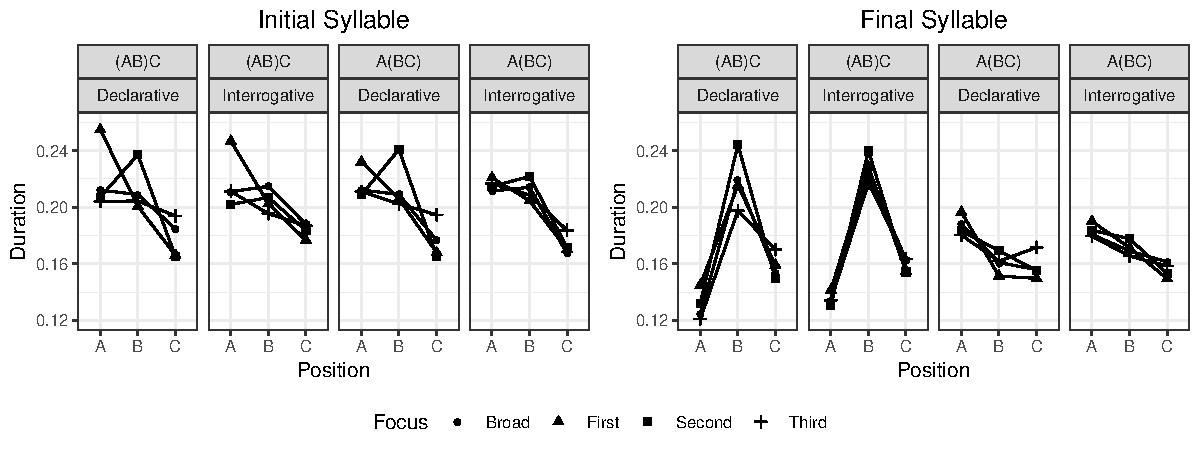
\includegraphics[width=5.4in]{Figures/syllable_duration.pdf}
		\caption{Duration (ms) of the initial and final syllable for each target word}
		\label{figureDuration}
	\end{center} 
\end{figure*}

When looking at the durational patterns in the final syllable in Fig. \ref{figureDuration}, the first pattern that catches the eye is that it closely tracks constituent structure. The plots of all of the combinations of focus and intonation are remarkably uniform for both left-branching and right-branching coordinate structures. If {\em A} forms a constituent with {\em B}, then the final syllable of A is much shorter and that of B much longer compared to the case in which {\em B} forms a constituent with {\em C}.  This makes sense if constituent structure maps to prosodic phrasing such that immediate conjuncts are phrased together to the exclusion of other constituents, and if the amount of lengthening on the final syllable correlates with whether the following constituent is in a separate phrase or in the same phrase. Notably, the durational effects of phrasing do not appear to be diminished by initial focus. This suggests, as was found already in \citet{norcl05}, that durational cues to phrasing remain intact in the post-focal domain. 

The plot of the durational effects on the initial syllable do not show any obvious correlates of phrasing or intonation, but they do show that duration provides cues for focus. At least in declarative utterances, the initial syllable of the focused word shows a boost in duration for all three focus conditions, compared to the baseline with broad focus. In the interrogative cases, this is only apparent when the initial constituent is focused (so for constituent A in the initial focus condition). The boost in duration of the focused initial syllable is much smaller on the final word C. \citet{coope85} also observed that final words show less focus-related lengthening compared to non-final words. Syllables other than the initial syllable of the focused word seem to be mostly unaffected by focus, and post-focal words for the most part do not show a reduction in duration. This again fits with \citet{coope85}, who similarly found that the effect of focus on duration is largely confined to the accented syllable of the focused word.\footnote{In our data, a small reduction in duration when post-focal is only observed for word C (but not for word B).} 

The plots suggest an interaction of focus with intonation: The different foci seem less differentiated by duration with interrogative intonation compared to with declarative intonation. 

In order to further evaluate the data, we fitted a regression model of the duration of initial and final syllables of word B, summarized in Table \ref{modelDuration}.\footnote{We focus here on measures of word B because based on the empirical plots, it seems like this is the most informative word. Looking at each word of interest would have made this paper too long. But of course analysis of the other words would also be of interest. We report additional models in the supplementary materials. We used the package lme4 (version 1.1-18-1) to fit the models, and estimated p-values with the package lmerTest \citep{kuzne13}.} The models we fit had duration (in seconds) as the dependent variable, and speech act, constituency, intonation, and their interactions as fixed effects. The model also included random slopes for all fixed effects, both for items and participants.  We estimated p-values using the Satterthwaite approximation to estimate the degrees of freedom \citep{kuzne13} (p-values were rounded to 0.001 or higher).


\begin{table}[h!]
\begin{center}
\begin{footnotesize}
\begin{tabular}{l D{)}{)}{11)3} D{)}{)}{11)3} }
\hline
 & \multicolumn{1}{c}{Initial} & \multicolumn{1}{c}{Final} \\
\hline
(Intercept)                                 & 0.21 \; (0.04)^{**}   & 0.19 \; (0.02)^{**}   \\
Broad.vs.Narrow                             & 0.00 \; (0.00)        & -0.00 \; (0.00)       \\
First.vs.Late                               & 0.01 \; (0.01)        & 0.00 \; (0.00)        \\
Second.vs.Third                             & -0.02 \; (0.01)^{***} & -0.02 \; (0.01)^{***} \\
Decl.vs.Inter                               & -0.00 \; (0.00)       & 0.01 \; (0.00)^{**}   \\
Left.vs.Right                               & 0.00 \; (0.00)        & -0.06 \; (0.01)^{***} \\
Broad.vs.Narrow:Decl.vs.Inter               & -0.01 \; (0.00)       & -0.00 \; (0.01)       \\
First.vs.Late:Decl.vs.Inter                 & -0.01 \; (0.01)       & -0.01 \; (0.01)^{*}   \\
Second.vs.Third:Decl.vs.Inter               & 0.03 \; (0.01)^{***}  & 0.01 \; (0.01)        \\
Broad.vs.Narrow:Left.vs.Right               & 0.01 \; (0.00)        & -0.00 \; (0.01)       \\
First.vs.Late:Left.vs.Right                 & -0.00 \; (0.01)       & 0.01 \; (0.01)        \\
Second.vs.Third:Left.vs.Right               & 0.00 \; (0.01)        & 0.02 \; (0.01)^{**}   \\
Decl.vs.Inter:Left.vs.Right                 & 0.00 \; (0.00)        & 0.00 \; (0.00)        \\
Broad.vs.Narrow:Decl.vs.Inter:Left.vs.Right & -0.00 \; (0.01)       & 0.00 \; (0.01)        \\
First.vs.Late:Decl.vs.Inter:Left.vs.Right   & 0.01 \; (0.01)        & -0.01 \; (0.01)       \\
Second.vs.Third:Decl.vs.Inter:Left.vs.Right & 0.00 \; (0.01)        & -0.03 \; (0.01)^{*}   \\
\hline
\multicolumn{3}{l}{\tiny{$^{***}p<0.001$, $^{**}p<0.01$, $^*p<0.05$}}
\end{tabular}
\end{footnotesize}
\caption{Mixed Effects Regression Models for the duration of word B (estimates in sec, SE in parentheses)}
\label{modelDuration}
\end{center}
\end{table}


The results for the initial syllable of word B show an effect of focus, such that with focus on B (second focus), the initial syllable was about 23ms longer than with focus on C ($\beta=-0.023; SE=0.005; t=-3.8; p<0.001$).\footnote{\citet{eady86} found a lengthening under focus of around 30ms.}  There was also a significant interaction with intonation ($\beta=0.026; SE=0.006; t=4.5; p<0.001$), indicating that this lengthening of the initial syllable due to focus was significantly smaller in questions.  

The results for the final syllable of word B also show a main effect of focus, similar in magnitude to that in the initial syllable ($\beta=-0.022; SE=0.005;-   t=-4.3; p<0.001$). There was also a main effect of intonation, such that the final syllable was significantly longer in questions ($\beta=0.096; SE=0.003; t=-3.1; p<0.005$), maybe because word B was typically realized with a rising pitch accent, and maybe realizing the rise required a longer final syllable. There was also a sizeable effect of phrasing, such that in the left-branching structure, the final syllable was significantly longer than in the right-branching structure ($\beta=-0.055; SE=0.008; t=-6.5; p<0.001$). In other words, the syllable was on average about 55ms longer when B was phrase-final and formed a constituent with A. There was also a small but significant interaction effect between first vs. late focus and intonation ($\beta=-0.012; SE=0.006; t=-1.97; p<0.05$), indicating that the choice of tune indeed significantly affected the realization of focus, with a smaller effect of focus in polar questions.\footnote{There were two further interactions effects, for which we do not have an interpretation: There was an interaction between the realization of Second.vs.Third focus and branchingness, and a three-way interaction between second vs. third focus, intonation, and syntactic constituent structure.}

If placing focus on A would erase the prosodic phrasing in the remainder of the utterance, then B should not vary depending on phrasing with first focus. An interaction between the effect of First.vs.Late Focus and branchingness (Left.vs.Right) could provide evidence for such a post-focal dephrasing effect. We did not, however, find evidence for such an effect. 


\subsection{Results: Intensity Effects}

Turning to intensity, Fig. \ref{figureIntensity} illustrates that the intensity of the final syllable provides a consistent cue to prosodic phrasing, across all conditions.  The observed effects of phrasing on intensity are a mirror-image of the duration effects: The final syllable of word A shows higher intensity than that of word B when they phrase together as a constituent, and lower intensity when they do not. This pattern cannot be explained by a simple gradual drop in intensity within phrases: The first constituent A, for example, should in that case always be realized in the same way across different phrasings. Instead, it seems that relative intensity is actively scaled to encode the prosodic phrasing of the utterance. 

\begin{figure*}[ht!]
	\begin{center}
		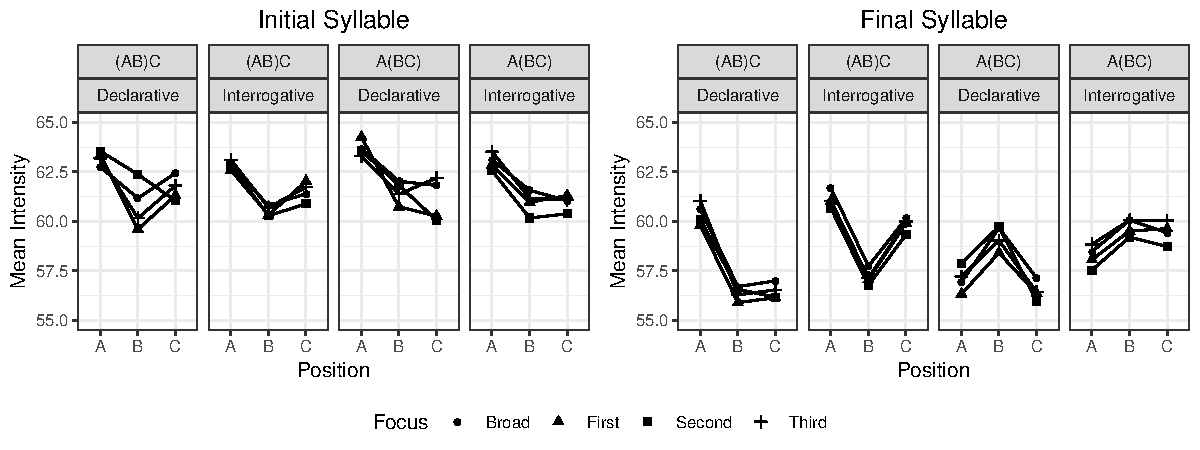
\includegraphics[width=5.4in]{Figures/Mean_Intensity.pdf}
		\caption{Mean intensity (dB) of initial and final syllable for each target word.}
		\label{figureIntensity}
	\end{center}
\end{figure*}

A second clear pattern in the plot is that the intensity of the final syllable of word C is higher in the interrogative condition compared to the declarative condition. This intensity increase may be an indirect consequence of the increased F$_0$ for the final rise. Increasing the rate of glottal fold vibration requires an increase in sub-glottal pressure, and may hence also result in greater intensity. Although intensity is typically not thought of as a cue to distinguish declarative and interrogative intonation, it seems clear that it is at least a reliable secondary cue in our data. 

The intensity pattern on the initial syllable is less clear. It seems that focus affects its intensity at least in the declarative condition, but the pattern is quite different depending on phrasing. The intensity of the initial syllable does not appear to vary by intonation. 

We again fitted models for word B to further evaluate the effects, which are reported in Table \ref{modelIntensity}.



\begin{table}[h!]
\begin{center}
\begin{footnotesize}
\begin{tabular}{l D{)}{)}{11)3} D{)}{)}{11)3} }
\hline
 & \multicolumn{1}{c}{Initial} & \multicolumn{1}{c}{Final} \\
\hline
(Intercept)                                 & 60.47 \; (1.36)^{***} & 57.69 \; (1.24)^{***} \\
Broad.vs.Narrow                             & -0.61 \; (0.16)^{**}  & -0.53 \; (0.21)       \\
First.vs.Late                               & 0.75 \; (0.24)^{*}    & 0.45 \; (0.29)        \\
Second.vs.Third                             & -0.38 \; (0.30)       & -0.15 \; (0.57)       \\
Decl.vs.Inter                               & -0.24 \; (0.29)       & 0.79 \; (0.43)        \\
Left.vs.Right                               & 0.73 \; (0.21)^{**}   & 2.73 \; (0.60)^{***}  \\
Broad.vs.Narrow:Decl.vs.Inter               & 0.20 \; (0.32)        & 0.27 \; (0.33)        \\
First.vs.Late:Decl.vs.Inter                 & -1.23 \; (0.35)^{***} & -0.57 \; (0.37)       \\
Second.vs.Third:Decl.vs.Inter               & 0.87 \; (0.40)^{*}    & 0.20 \; (0.42)        \\
Broad.vs.Narrow:Left.vs.Right               & -0.42 \; (0.32)       & -0.04 \; (0.33)       \\
First.vs.Late:Left.vs.Right                 & -0.68 \; (0.35)       & 0.14 \; (0.37)        \\
Second.vs.Third:Left.vs.Right               & 0.52 \; (0.40)        & -0.30 \; (0.41)       \\
Decl.vs.Inter:Left.vs.Right                 & 0.05 \; (0.28)        & -0.19 \; (0.30)       \\
Broad.vs.Narrow:Decl.vs.Inter:Left.vs.Right & -0.72 \; (0.64)       & -0.47 \; (0.67)       \\
First.vs.Late:Decl.vs.Inter:Left.vs.Right   & 0.35 \; (0.71)        & -0.31 \; (0.73)       \\
Second.vs.Third:Decl.vs.Inter:Left.vs.Right & -1.17 \; (0.80)       & 0.60 \; (0.83)        \\
\hline
\multicolumn{3}{l}{\tiny{$^{***}p<0.001$, $^{**}p<0.01$, $^*p<0.05$}}
\end{tabular}
\end{footnotesize}
\caption{Mixed Effects Regression Models for the mean intensity of word B (estimate in dB, SE in parentheses).}
\label{modelIntensity}
\end{center}
\end{table}


For the initial syllable, there was a significant effect of First.vs.Late focus, such that the initial syllable of word B had lower intensity if the first conjunct was focused ($\beta=0.75; SE=0.24; t=3.1; p<0.05$). This is as expected if words are reduced in intensity post-focally.\footnote{There was also a significant effect of Broad.vs.Narrow, such that the initial syllable of word B was longer under narrow focus compared to the control condition ($\beta=-0.61; SE=0.16; t=-3.8; p<0.002$). We would have expected that the comparison between Second.vs.Third would be significant instead.}

There was an effect of similar size of phrasing  ($\beta=0.73; SE=0.21; t=3.5; p<0.02$), indicating that the intensity of the initial syllable of word B was `scaled' to encode the constituent structure: B had lower intensity when it was phrase-final (in the left-branching structure), compared to when it was phrase-initial (in the right-branching structure). There were furthermore two interaction effects between how focus was realized and the choice of intonation, suggesting that intensity was a significantly less reliable cue for focus in interrogative utterances.

For the final syllable, there was only one significant effect. The final syllable of word B, just like its initial syllable, showed a lower intensity in the left-branching structure, where it was phrase-final,  compared to the right-branching structure, where it was phrase-intial ($\beta=2.73; SE=0.6; t=4.5; p<0.001$).  

If focus on the first constituent were to obliterate phrasing later, then we would expect an interaction between First.vs.Late and Left-vs.Right. We did not find evidence for such an interaction.


\subsection{Results: F$_0$ Effects}

In declaratives, focus clearly affects the F$_0$-pattern of the initial syllable of the target words. The initial syllable of a focused word is generally boosted compared to the broad focus baseline for all three target words A, B, and C.  This replicates similar effects reported in \citep[][i.a.]{breenetal10}.\footnote{Interestingly, \citet{eady86} found no boost in pitch for initial constituents. A relevant difference to our study is, however, that our target sentence was not the only clause the participants produced. Word A was clause-initial, but not utterance-initial, while in their study the initial word of interest they looked at was utterance-initial.} There was one exception, however: With third focus, in the left-branching structure, the pitch on the initial syllable of the focused word C is similar to the baseline.\footnote{Maybe relatedly, \citet{eady86} report that pitch was boosted on the final word with late focus, while \citet{coope85} report that this is not the case in longer utterances, where the maximum pitch is similar to baseline in this case. It's not clear why our left-branching (as opposed to right-branching) cases should pattern with the longer sentences in their studies, but it is interesting that a similar point of variation was observed before.}

The pitch of the initial syllable appears to be systematically lowered when a word is post-focal, such that the initial syllable of B is lower compared to baseline when A is focused, and the initial syllable of C is lowered when A or B are focused. By contrast, there is only little evidence for pre-focal reduction: Pitch on the initial syllable of word A is comparable to baseline when focus is placed on B and C; pitch on the initial syllable of word B is only reduced for third focus in the left-branching structure, but is identical to baseline in the right-branching structure. Earlier studies also found that pitch reduction is stronger post-focally compared to pre-focally \citet{eady86,eady86dual}, an observation to which we return when looking at human annotations of the data in the next section.


\begin{figure*}[ht!]
	\begin{center}
		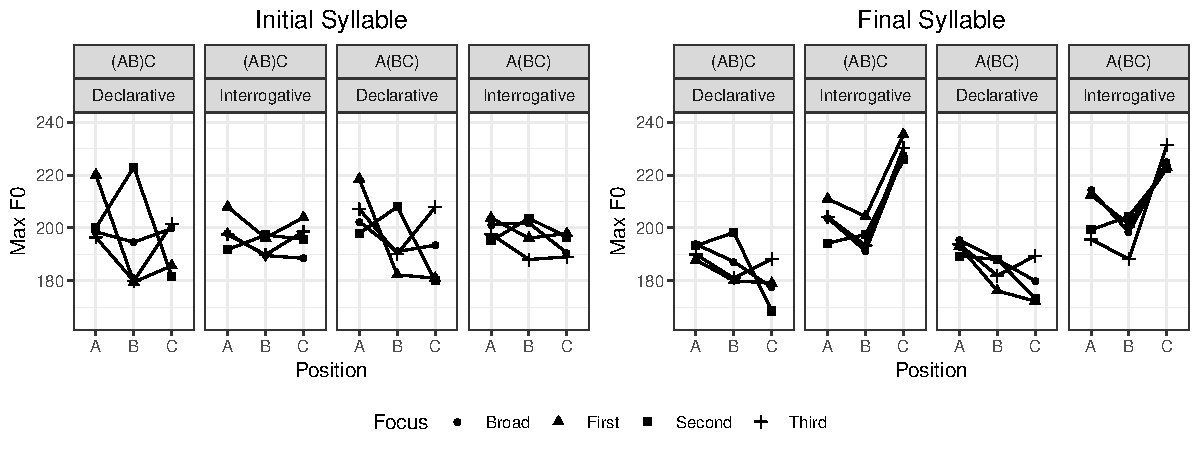
\includegraphics[width=5.4in]{Figures/Max_F0.pdf}
		\caption{Mean F$_0$ (Hz) of initial and final syllable for each target word}
		\label{figurePitch}
	\end{center}
\end{figure*}

 Systematic effects of phrasing and intonation are not apparent for the initial syllable. The pattern of F$_0$ on the final syllable, however, shows clear effects of the intonational contour: The pitch of the final syllable of word  C is substantially higher in interrogatives, reflecting the final high boundary tone of the question contour. F$_0$ on the final syllable of word A and B appears to be higher in interrogatives as well, compatible with these words carrying rising accents. The effects of focus and phrasing on the final syllable seem comparatively weak, if present at all.

We again fitted a regression model for word B, reported in Table \ref{modelPitch}. The model for the initial syllable shows a significant effect of First.vs.Late focus, confirming that the initial syllable of word B was indeed significantly reduced (by about 10Hz) when the first word was focused ($\beta=9.6; SE=3.2; t=-3.0; p<0.007$). There was also a significant effect of Second.vs.Third focus, confirming that pitch of the initial syllable of word B was significantly boosted when it was focused ($\beta=-19.4; SE=4.8; t=-4.0; p<0.001$). There were also highly significant interactions of focus with intonation (First.vs.Second:Decl.vs.Inter and Second.vs.Third:Decl.vs.Inter), showing that focus was cued less reliably in questions.\footnote{There was also a significant interaction between intonation and branching, as well as a significant three-way interaction, for which we do not have an interpretation.}


\begin{table}[h!]
\begin{center}
\begin{footnotesize}
\begin{tabular}{l D{)}{)}{12)3} D{)}{)}{12)3} }
\hline
 & \multicolumn{1}{c}{Initial} & \multicolumn{1}{c}{Final} \\
\hline
(Intercept)                                 & 192.50 \; (7.77)^{***} & 189.56 \; (8.45)^{***} \\
Broad.vs.Narrow                             & 0.88 \; (3.11)         & -0.13 \; (1.70)        \\
First.vs.Late                               & 9.63 \; (3.25)^{**}    & 1.93 \; (4.26)         \\
Second.vs.Third                             & -19.41 \; (4.81)^{***} & -11.01 \; (4.69)       \\
Decl.vs.Inter                               & 1.46 \; (3.27)         & 12.23 \; (4.51)^{*}    \\
Left.vs.Right                               & 2.40 \; (2.06)         & 0.16 \; (2.19)         \\
Broad.vs.Narrow:Decl.vs.Inter               & 1.05 \; (3.22)         & 9.88 \; (3.41)^{**}    \\
First.vs.Late:Decl.vs.Inter                 & -18.61 \; (3.53)^{***} & -12.58 \; (3.78)^{***} \\
Second.vs.Third:Decl.vs.Inter               & 18.88 \; (4.04)^{***}  & 0.58 \; (4.29)         \\
Broad.vs.Narrow:Left.vs.Right               & -1.98 \; (3.21)        & -4.03 \; (3.41)        \\
First.vs.Late:Left.vs.Right                 & -3.67 \; (3.53)        & -0.24 \; (3.78)        \\
Second.vs.Third:Left.vs.Right               & 5.87 \; (4.01)         & -1.47 \; (4.26)        \\
Decl.vs.Inter:Left.vs.Right                 & 5.96 \; (2.85)^{*}     & 3.35 \; (3.04)         \\
Broad.vs.Narrow:Decl.vs.Inter:Left.vs.Right & -9.62 \; (6.42)        & 1.86 \; (6.82)         \\
First.vs.Late:Decl.vs.Inter:Left.vs.Right   & 7.19 \; (7.06)         & 0.95 \; (7.57)         \\
Second.vs.Third:Decl.vs.Inter:Left.vs.Right & -19.07 \; (8.02)^{*}   & -9.16 \; (8.54)        \\
\hline
\multicolumn{3}{l}{\tiny{$^{***}p<0.001$, $^{**}p<0.01$, $^*p<0.05$}}
\end{tabular}
\end{footnotesize}
\caption{Mixed Effects Regression Models for the Max F$_0$ of word B (estimate in Hz, SE in parentheses).}
\label{modelPitch}
\end{center}
\end{table}


For the final syllable, there was an effect of intonation ($\beta=-12.59; SE=3.9; t=3.2; p<0.01$). There were also interactions between First.vs.Late Focus and Second.vs.Third Focus. Notably, there were no significant effects of phrasing on pitch in either syllable.


\section{Discussion}
% The discussion should start to interpret the results, i.e. give the relation between the raw acoustic measures and their phonological interpretation, again, best way would be to structure the discussion along the hypotheses

Our results show that duration, intensity, and pitch are all affected by each of the three functional dimensions, constituent structure, focus, and speech act. %These dimensions arguably exert their influence indirectly via their effects on prosodic phrasing, (focus) prominence, and intonation. 
There are two patterns that make it easier to tease apart the three dimensions, despite the overlap in which acoustic cues they affect. The first is that the three dimensions tend to affect different syllables. Focus prominence mostly affects the accented syllable, constituent structure mostly affects the final syllable, and intonation affects both. 

The second pattern is that the the acoustic cues have different relationships with each other depending on the dimension. For example, duration, pitch and intensity of the initial syllable all increase when a word is focused; however, when a word  is phrase-final, duration increases while intensity {\em decreases} (and we did not find a pitch effect). In other words, the cues mutually inform each other about the which dimension is being cued. A listener can draw different conclusions depending on whether increase in duration is accompanied by an increase in intensity or a decrease.\footnote{This difference in relation with each other may be at the heart of the interaction-effect observed between duration and intensity in the logistic regression fitted to predict prominence judgments in \citet{bisho19}.}

Our main research question was whether focus prominence obliterates cues to phrasing in the post-focal domain. Our data show no evidence for this. Based on the empirical plots, the duration of the final syllable of our target words consistently reflect phrasing, unperturbed by variation in focus or intonation. The intensity of both the (accented) initial syllable and the final syllable also varies by phrasing. We found main effects of phrasing for several of our measures, but for no acoustic measure did we find an interaction between the effect of constituency and the effect of focus. There is no evidence therefore that focus erases or diminishes phrasing distinctions in the post-focal domain. 

In addition, we found that focus is cued less reliably with interrogative intonation. It seems then that question intonation tends to diminish cues to focus at least to some extent.  We explore these two findings in more detail the next section. This differs from findings in \citet{eady86}, where the choice between declarative intonation and question intonation did not affect the durational cues to focus, no interaction with intonation was observed. An important difference in their study, however, is that when the experimenter thought that focus was not successfully conveyed prosodically, speakers were instructed to rerecord a sentence. In the next section, we use the effect of intonation on focus in our data as a point of comparison to evaluate whether there might be an effect of focus on phrasing that remained undetected by our models. Before doing so,  we want to take stock of a few findings that are not our main focus, but are nevertheless of interest. 

An interesting parallel in our results to those of \citet{coope85} and \citet{eady86} is that while durational cues to focus are confined (largely) to the accented syllable of the focused word, the pitch cues to focus are more globally distributed, since post-focal material is also affected. Our results furthermore show that in this regard intensity patterns more similarly to pitch, in that post-focal material is also reduced in intensity.

Furthermore, we observed an interesting pattern regarding the phrasing-related lengthening effect that affects the last syllable of a word. We found a much greater effect of final lengthening in pre-boundary environments, when another conjunct followed, compared to the final conjunct. This replicates similar findings in \citet{wagner05recursion}, and suggests that these are planning-related pre-boundary effects rather than (just) effects of final lengthening. Note, however, that in our utterances there was material following the final conjunct, which was contextually given and hence unaccented, which may explain why the observed final lengthening in word C was not greater.\footnote{A reviewer points out that the reason for the increased effect coordinate-structure internally could be that speakers are trying to disambiguate the globally ambiguous structure. Our data do not allow to test whether this is the case. Another reviewer suggests that there may be greater lengthening phrase-internally because there may be no clear tonal cue signalling the phrase boundary while intermediate-phrase finally, there is a boundary tone. See \citet{gollr13} for evidence that pitch only plays a minor role in cueing intermediate phrase boundaries in German.} 

This result relates to the comparatively small degree of lengthening for focus reasons we found in the final word: \citet{coope85}, similarly,  found that final words show less of a durational increase under focus, an attribute this finding to a ceiling effect---the final word is subject to final lengthening for phrasing reason, and hence cannot expand much to also encode focus. This explanation does not seem applicable in our case:  Since we didn't find evidence for phrasing-related  lengthening in the final word, there is no reason to assume that a ceiling in duration was reached. Also, it is not clear why a ceiling should be reached for lengthening the initial syllable anyway, when phrase-related lengthening mostly affects the final syllable. This casts doubt on an explanation based on overall expandability. An alternative interpretation of the smaller focus effect on the last word is that the last accented word is perceived as sufficiently prominent for a focused word simply by virtue of being last, making it less important to mark late focus phonetically. 

Another interesting finding is that phrasing seems to be reliably cued by intensity-scaling. Both the initial accented syllable and the final unaccented syllable show clear effects of phrasing, such that there is higher intensity at the beginning of phrases and lower intensity later in phrases. There is clear evidence that these effects go beyond a drop in sub-glottal pressure due to exhalation throughout the utterance or throughout phrases. We would not expect to see a difference in the intensity on the first constituent (A) if this were the case. And yet, Fig. \ref{figureIntensity} illustrates that A varies in intensity depending on whether it phrases with B or not. It seems then that intensity-scaling is actively used to encode prosodic phrasing in ways that go beyond the downdrift throughout the utterance. This is compatible with related findings in German reported in \citet{poschmannwagner16}.  

The lack of pitch accent scaling effects due to phrasing, and the clear presence of intensity-scaling, is compatible with the hypothesis that intensity is a primary cue for phrasing, while apparent effects of pitch-accent scaling observed in the earlier literature may really have been an indirect side-effect of intensity scaling.  Intensity in speech closely correlates with pitch \citep{gramm88}. The correlation with pitch is not a physical necessity, of course, and individuals seem to have independent control over the two cues---we are able in principle to talk louder or quieter without changing F$_0$.  And yet, when asked to speak louder, speaker spontaneously often raise their pitch. It seems that an increased sub-glottal pressure will result higher vocal fold vibration unless we prevent this from happening. The close correlation between the two cues opens the possibility that pitch may be used to enhance an intended intensity effect and vice-versa. Maybe pitch accent scaling is only an indirect correlate of intensity scaling. Further investigation of this idea is needed. Our results minimally suggest that intensity-scaling is a stronger and more reliable cue to phrasing than pitch-scaling. In our data, pitch appears not to be a good to cue to phrasing, even in the case of broad focus.

Pitch cues to differences in phonological phrasing were also not found to be very relevant in the perception studies conducted in \citet{gollr13} on German.  However, \citet{gollr13} found that pitch cues related to boundary tones were much more relevant to cue intonational phrasing than in phonological phrasing. It seems plausible that in our data, intonational phrase breaks were used less frequently than phonological phrase boundaries to mark the intended phrasing, given the shortness of the conjuncts. Maybe we would have found reliable pitch cues if we had looked at phrasing distinctions among larger constituents that map to intonational phrases, as \citet{ladd88} did in his classic study on pitch scaling. 

Overlay models predict the prosodic reflexes of the three separate dimensions to be independent and recoverable from the signal, while most current phonological models predict interactions resulting in neutralizations between conditions. We found no evidence that phrasing distinctions are neutralized in the post-focal domain. The plots suggest that focus and phrasing are, for the most part, encoded independently of each other, as expected by overlay models. It should be noted  that such additive effects of different factors are not inherently incompatible with AM-models {\em in principle}. \citet[18]{pierr80}, for example, anticipates that the expressive use of pitch of a speakers trying to `highlight' certain parts of the utterance might `multiplicatively determine the F$_0$ value of a given tone'.  We will discuss particular proposals about phonological presentations compatible with our findings in section \ref{twoprom}. 

How compelling is the evidence that the prosodic cues to phrasing and focus are orthogonal to each other? The lack of significant interaction effects is only of limited informativeness. We cannot rule out that our experiment was simply not powerful enough to detect such effects. At least the empirical plots show highly consistent patterns across conditions, and make it seem implausible that focus has radical effects on post-focal phrasing. We can do better, however. In the next section, we will try to quantify just how well various acoustic cues convey phrasing, and also how much loss of information there is when focus is placed early. This will also address a second worry one may have based on the results reported above: By looking only at a few acoustic cues from the second conjunct (word B), we have used a very limited amount of information from the signal. 


\section{How well is phrasing cued post-focally?}
\label{forest}

In order to evaluate to what extent information about phrasing in the post-focal domain is lost, we need to find a way to look at many acoustic cues at the same time, and evaluate how they fare in cueing phrasing for different focus conditions. One way we can accomplish this is by automatically classifying the data given a set of acoustic features. There are many different types of classifying algorithms. Here, we will use Random Forests \citep{breim01,strob09}. Random forests have been used insightfully in earlier work in linguistics \citep{tagli12,tao18,bauma18}, including in this special issue \citep{wagne19}. 


\subsection{Methods}

Random forests provide a non-parametric statistical tool which allows us to evaluate a set of features (a `feature space') in its usefulness in classifying observations into pre-set categories. Compared to alternative analysis methods, they have the advantage of being robust with respect to collinearity among the predictors, and in being compatible with a large set of predictors with a relatively low $n$ \citep{strob09}. The former property is important if one wants to explore the contributions of both pitch and intensity, since they are generally highly correlated, as noted before. 

A random forest consists of an `ensemble' or `forest' of classification and regression trees (CART, \citealt{breim84}). The trees in the forest vary in which subset of the data they were trained on, and which subset of predictors were used. CARTs classify the data by recursive splits that try to optimally sort the data into the correct bins. A disadvantage of CARTs is that the ranking of predictors is very sensitive to small changes in the data used to train them. Each split at a given point  in the classification tree is very sensitive to the particular training data, and can have large downstream effects on which features will be chosen. If different subsets are used to train a CART, very different classification trees may emerge. In any given tree, a particular predictor may be masked by others, even if, when faced with novel data, that predictor might have been very useful. Similar issues can arise in stepwise predictor-selection algorithms in logistic regression models. Random forests avoid this issue by fitting many CARTs based on different subsets of the data.  One can then evaluate the importance of particular predictors over the entire forest. In addition, they increase the variability of trees even further by restricting the set of predictor variables for each individual tree, which helps to estimate their relative usefulness even more accurately. 

Random forests have two parameters, the number of trees (`ntree'), and the number of randomly preselected splitting variables for each tree (`mtry'). Small data sets may require a larger number of trees to find robust results. A low number of `mtry' increases tree diversity. This is because we select a small number of predictors, it is more likely that more  important features are missing, which will give the `lesser' features an opportunity to show their worth. However, it leads to more trees in which all relevant predictors are left out, introducing more noise. A high value for this parameter means that the best predictors will usually be chosen, and thus tree diversity decreases,  and along with it the quality of information gained on lesser features \citep[for more discussion, see][]{strob09}. 

Random forests have two more useful properties. First, they allow us to estimate how well a set of features differentiate different categories by testing how well data is classified that was left out of the training set for each tree during the training phrase. This is called `out-of-bag' (OOB) prediction. Second, they allow us to evaluate the relative importance of particular predictor variables. This is done by permuting the values of particular predictors and evaluating how this affects the classification accuracy on out-of-bag data. If a predictor is important for the classification, permuting its value will greatly affect out-of-bag classification accuracy. If it was involved in a tree by chance, then it will not. These permutations yield variable importance measures for each predictor. The absolute values of these importance measures are hard to interpret, but the relative ranking is meaningful. It tells us which features were most important in the model. If a variable has an importance close to zero, it does not contribute much to the accuracy of the predictions. If it is negative, then leaving it out of a classification tree improves the classification. 

In order to first understand which predictors were important to encode focus, we fitted a random forest to predict the original focus context that an utterance was uttered in. The predictors included duration, pitch, and intensity measures for each of the three target words for each syllable, for a total of 18 measures.  Following the heuristic in \citet{strob09}, we set the parameter mtry to the rounded square root of the number of predictors (mtry=4). We used forests of 1000 trees. We also ran the analysis with different parameters (mtry=3 \& 5, ntrees=5,000) to ensure that the results are stable.\footnote{We used the R {\em party}-package to compute the random forest analysis \citep{hotho06,strob07,strob08}. Apart from the cited literature, we also thank Stephanie Shih and Francisco Torreira for their useful class materials on random forest analysis.}

In analysis based on mixed models, we have seen that focus seems to have had less of an effect in interrogative utterances. Therefore, we ran the analysis not just on the entire data, but also on the subset of declarative utterances and interrogative utterances respectively, in order to assess how the choice of intonation affected the accuracy of the classification. The goal was to see how much information about  focus is still present in the interrogative utterances, compared to the declaratives. We then proceeded to look at our central question, which is how much information about {\em phrasing} is lost in the post-focal domain, and fitted a random forest model to predict phrasing. Here, we were interested whether the classification accuracy was lower when focus was initial compared to the case of broad focus---if initial focus adversely affects cues to phrasing, the the classification for phrasing should be lower.


\subsection{Results}

Table \ref{focusForestTable} illustrates how well the random forest performed compared to a human annotator, tasked with guessing which focus condition an utterance was recorded in.\footnote{We do not report the accuracy on the training data since these accuracy percentages are inflated, and will not reflect how well the model would do when encountering new data. %For example, the accuracy of predictions overall for Focus is 83.1\%, but the accuracy of the OOB-predictions is 34.9\%.
}

\begin{table}[ht]
\centering
\begingroup\footnotesize
\begin{tabular}{rllll}
  \hline
 & Focus & R.F./Annotator--All & R.F./Annotator--Dec & R.F./Annotator--Int \\ 
  \hline
1 & Broad & 0.26/0.16 & 0.33/0.14 & 0.19/0.16 \\ 
  2 & First & 0.4/0.35 & 0.43/0.39 & 0.28/0.26 \\ 
  3 & Second & 0.38/0.36 & 0.45/0.45 & 0.26/0.24 \\ 
  4 & Third & 0.37/0.6 & 0.31/0.66 & 0.21/0.49 \\ 
   \hline
\end{tabular}
\endgroup
\caption{Proportion of accurate classification for all data, declarative  data (Dec), and interrogative data (Int). For each data set, both the accuracy of the random forest classification (R.F.), as well as of the human annotation is given.} 
\label{focusForestTable}
\end{table}


For the declaratives, the random forest classifier has an accuracy between  31\%  and 44\%. This is not spectacular, but much better than chance, which is at 25\%. The accuracy is much better for those foci where a prominence shift is predicted, that is, where the last accent does not fall on the last name ($>40\%$). The accuracy for broad focus and third focus is substantially lower ($<31\%$). The annotator also was susceptible to this, and often confused broad and third focus, showing a strong bias to annotate third focus over broad focus.  For the interrogatives, the accuracy for all foci is much lower ($<30\%$), and close to chance. 

Fig. \ref{FocusForest} shows the ranking of the importance of the predictors based on the permutation score on out-of-bag accuracy. The solid black line shows zero---a predictor of an importance score close to zero does not contribute much to the accuracy of the model. The dashed line plots the absolute value of the lowest negative predictor. Any predictor to the right of this line plausibly contributes to the model, while predictors to the left probably do not: Since non-informative predictors will have random importance scores fluctuating around zero, the absolute value of the lowest predictor is often taken an approximate cut-off  to distinguish predictors that contribute information and predictors that do not \citep{strob09}. F$_0$ of the initial syllable and duration of the first and final syllable appear to be the best cues to focus in the declarative data. 


\begin{figure*}[ht!]
	\begin{center}	     
	       %\parbox{2.1in}{All data:\\
	       %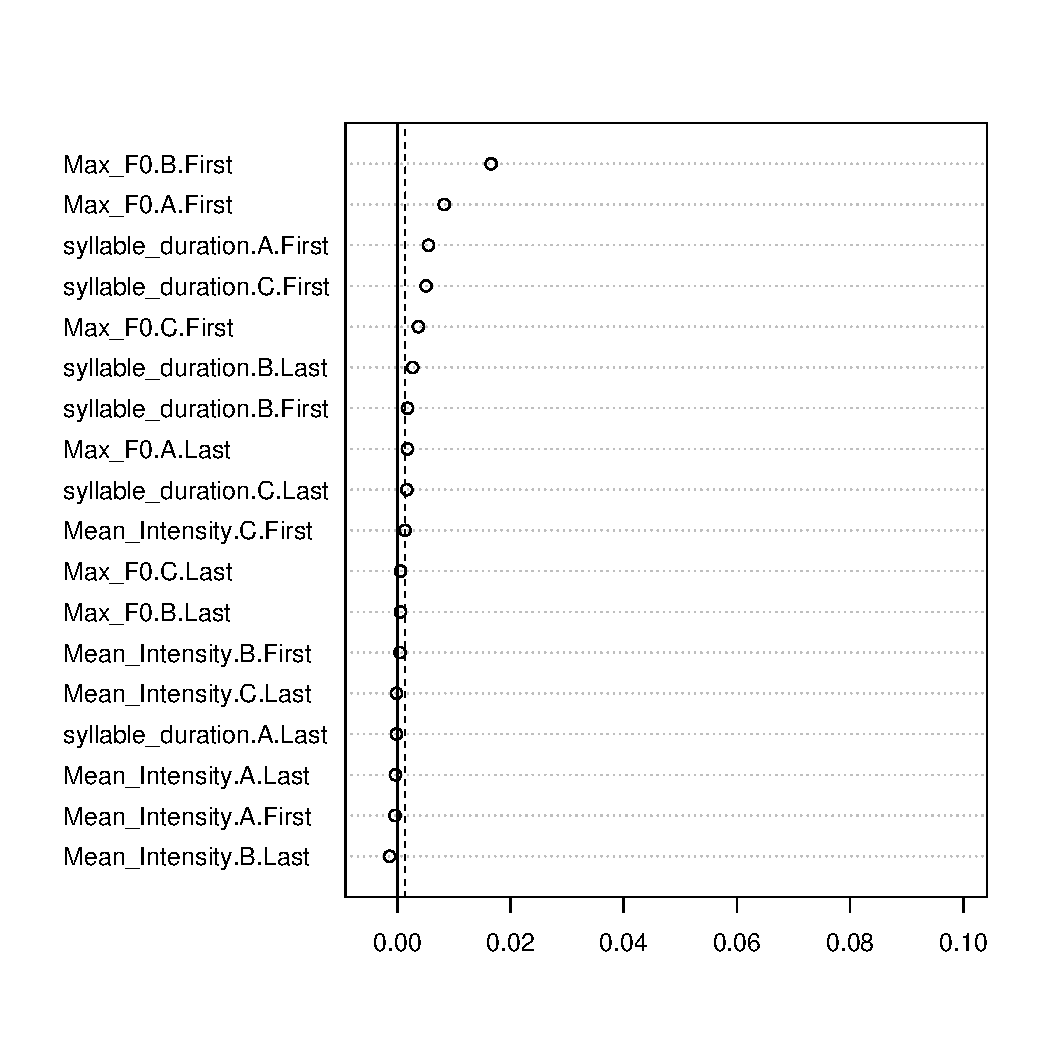
\includegraphics[width=2in]{Figures/FocusVarimp.pdf}
	       %}
	        \parbox{2.8in}{
		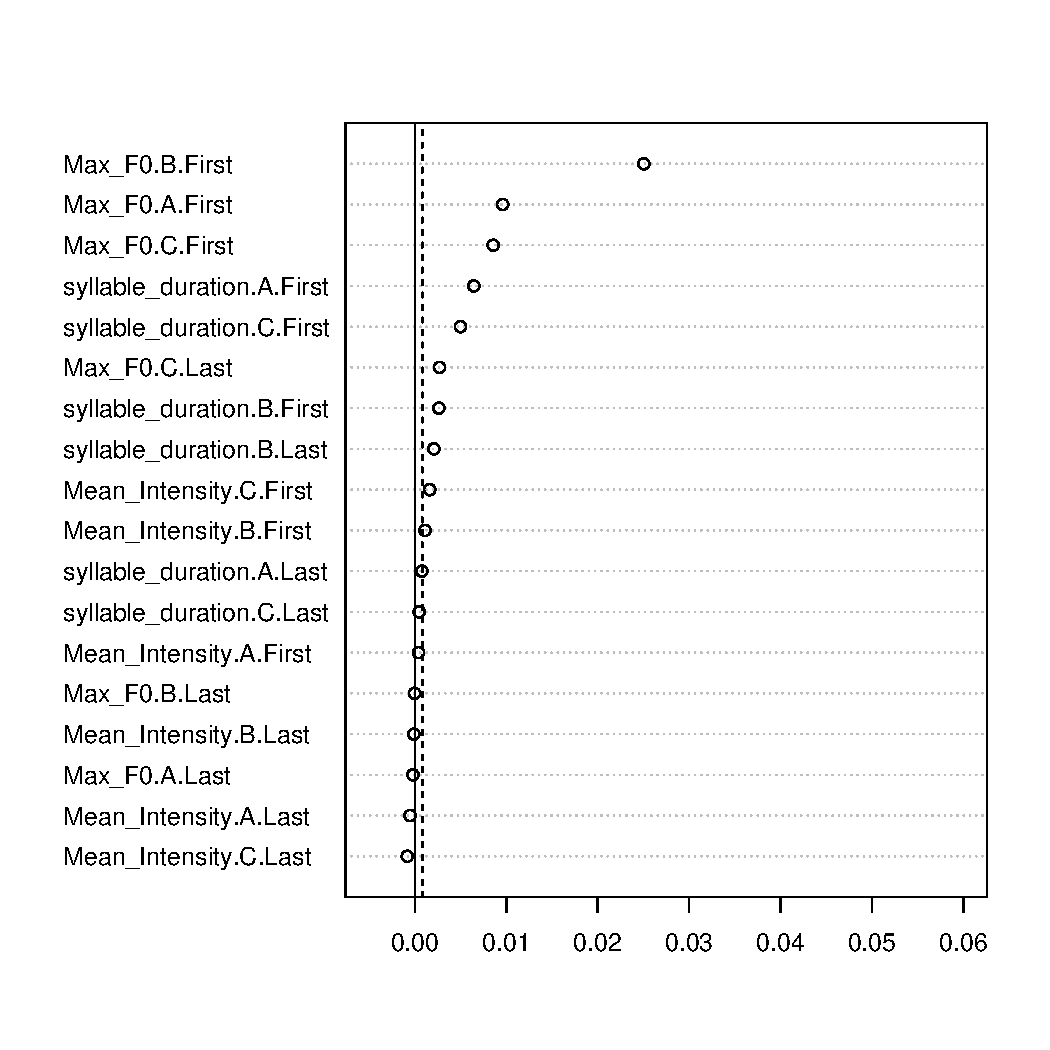
\includegraphics[width=2.8in]{Figures/FocusVarimpDec.pdf}
		}\parbox{2.8in}{
		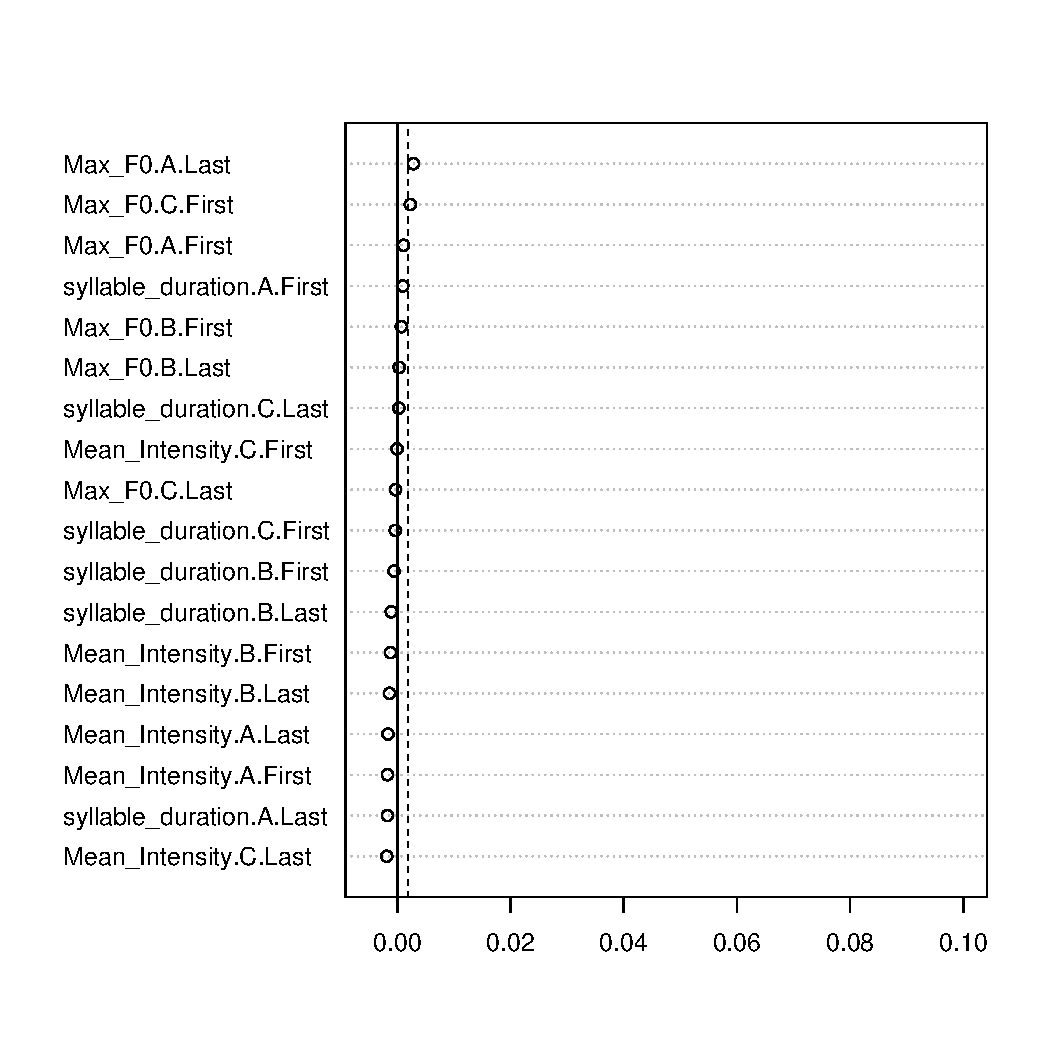
\includegraphics[width=2.8in]{Figures/FocusVarimpInt.pdf}
		}
	     \caption{Importance of variables in random forest classification of Focus for the Declarative (left) and the Interrogative (right) utterances respectively}
	     \label{FocusForest}
	\end{center}
\end{figure*}

For the interrogative data, random forests are roughly at chance, and it seems that focus is simply not systematically encoded. 

Having established the cues to focus prominence, let's now look at phrasing. Again we applied the random forest analysis on three different sets of data: the entire data set, the subset only consisting of broad focus, and the subset only consisting of focus on the first constituent and for which the annotators were able to hear first focus correctly. The latter data set is the one where we should see information about phrasing lost if phrasing cues are indeed adversely affected in the post-focal domain. The accuracy of the out-of-bag predictions are plotted in Table \ref{phrasingForestTable}.

\begin{table}[ht]
\centering
\begingroup\footnotesize
\begin{tabular}{rllll}
  \hline
 & Constituency & R.F./Annotator--All & R.F./Annotator--Broad & R.F./Annotator--First \\ 
  \hline
1 & (AB)C & 0.8/0.61 & 0.78/0.63 & 0.74/0.6 \\ 
  2 & A(BC) & 0.75/0.62 & 0.76/0.61 & 0.79/0.63 \\ 
   \hline
\end{tabular}
\endgroup
\caption{Proportion of accurate classification for all data, broad focus data, and first focus data. For each data set, both the accuracy of the random forest classification (R.F.) and the human annotation is given.} 
\label{phrasingForestTable}
\end{table}


The results show that the RF classification in all three data sets was comparable: In the classification on the left-out data they all performed at or above 74\% (where chance is 50\%). Crucially the classification worked just as well for the data set with initial focus. The human annotators performed more poorly than the RF model, but still better than chance, at an accuracy of 0.6 or above. Again, the accuracy of branching was not lower in the data set with initial focus.

Fig. \ref{phrasingForest} shows the relative importance of the predictors for the classification of phrasing. For both broad and first focus data, the same acoustic features did most of the work, namely the duration and intensity of the final syllable. There is also some evidence that the pitch of the accented initial syllable is relevant, but it only makes a small contribution to the classification, and the importance of this measure drops in the post-focal domain. 


\begin{figure*}[ht!]
	\begin{center}
	{\footnotesize
	    % \parbox{2.1in}{All data:\\
	    %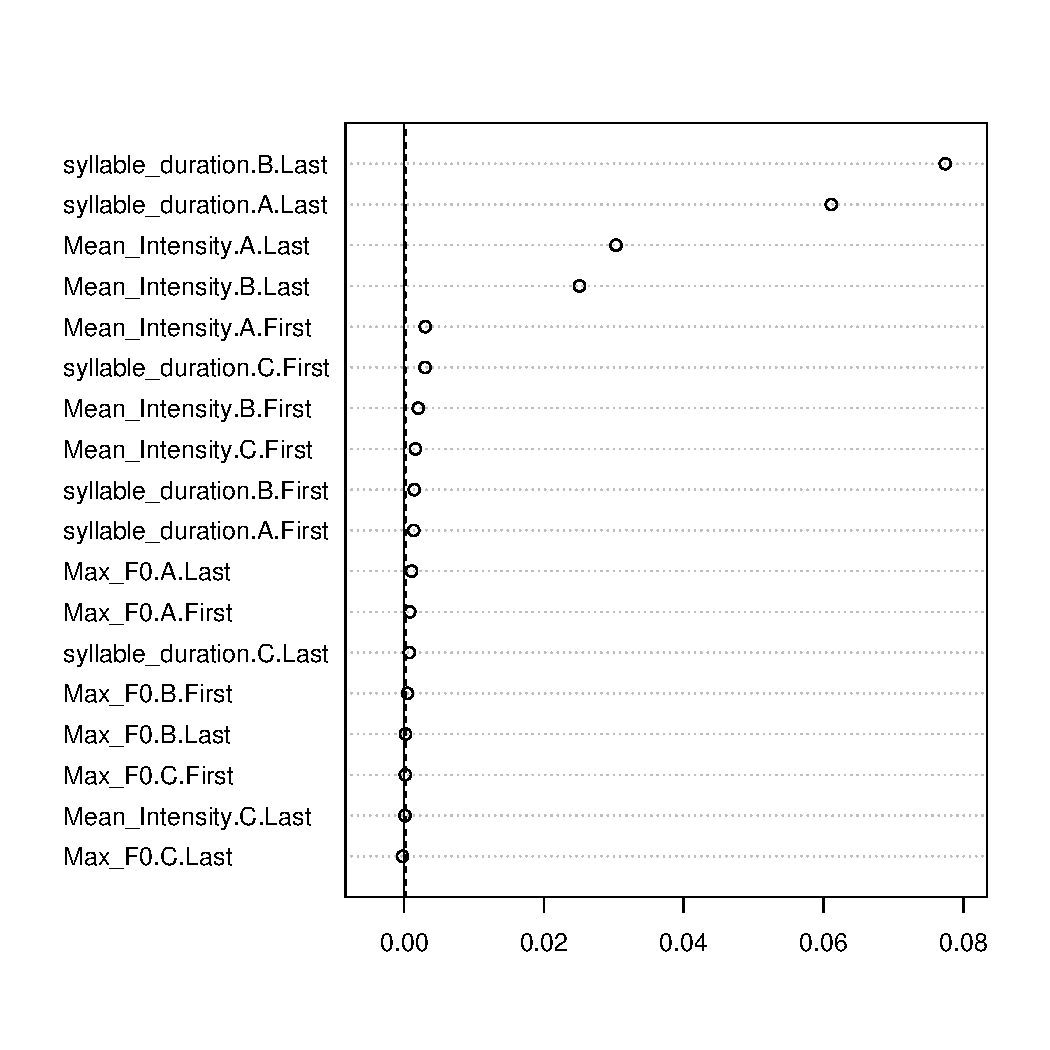
\includegraphics[width=2in]{Figures/phrasingVarimp.pdf}
	     %}
	        \parbox{2.8in}{
		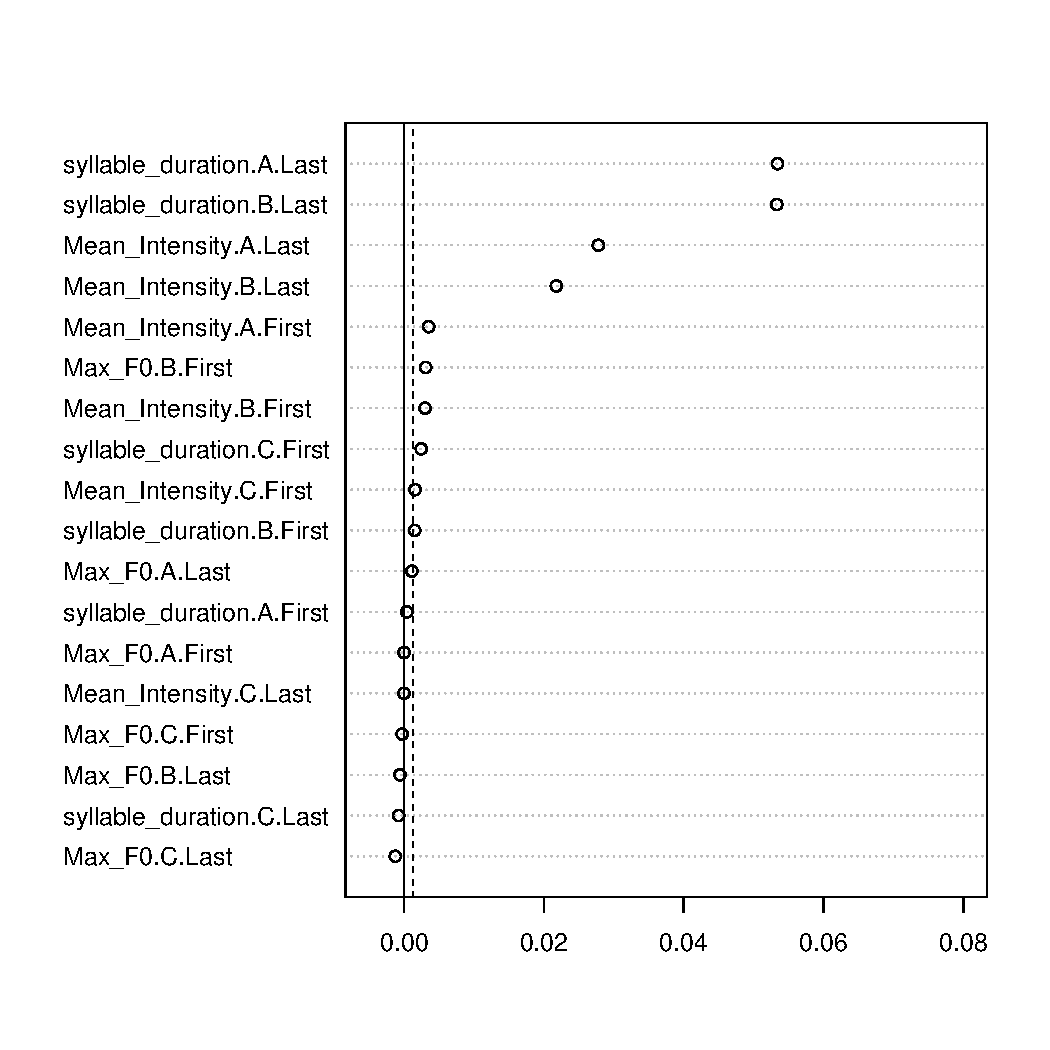
\includegraphics[width=2.8in]{Figures/phrasingBroadVarimp.pdf}
		}\parbox{3.5in}{
		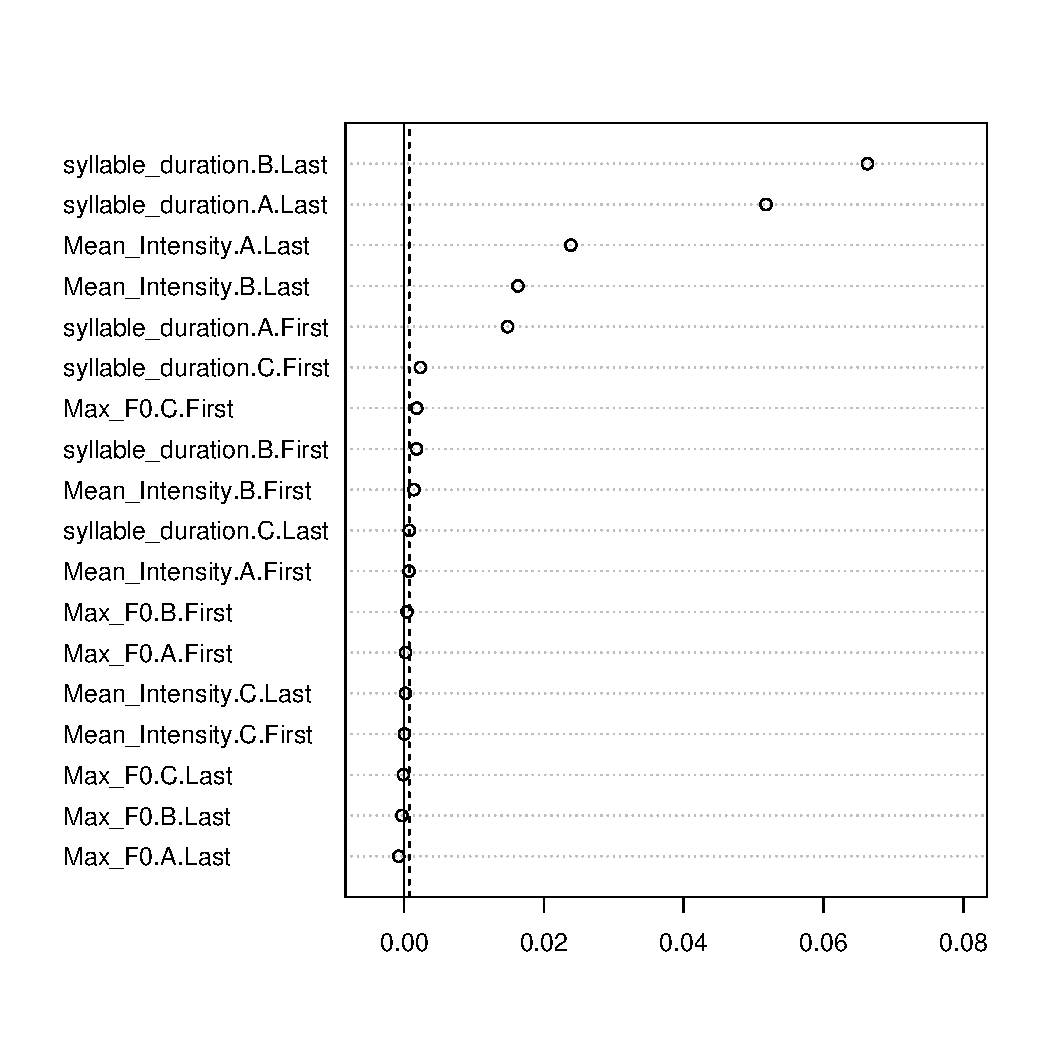
\includegraphics[width=2.8in]{Figures/phrasingFirstVarimp.pdf}
		}
		}
		\caption{Importance of variables in random forest classification of Constituency for the case of broad focus (left) and first focus (right) respectively}
		\label{phrasingForest}
	\end{center}
\end{figure*}


\subsection{Discussion}
\label{twoprom}

The random forest analysis for focus confirmed what we already anticipated given the empirical plots and the regression models: Focus was cued less reliably in interrogatives. The random forest analysis added further information, however, regarding how well the information was cued. For the most part, it seems that only first focus was encoded with any success in the interrogative condition, and even in that condition it was close to chance. The human annotators were not much better than the random forest models, which suggests that we didn't simply feed the model the wrong acoustic measures. 

These results are somewhat surprising, since it is clearly possible in principle to mark focus in questions. For example, focus is clearly conveyed in the interrogative utterances we used for illustration in \ref{examm2}. Based on our own perception of the data, it seems to us that in the interrogative condition, speakers often simply didn't bother to mark focus. This may show that focus marking in interrogatives is less obligatory than in declaratives. Given the high correlation of tune and function, it is not clear whether this is due to the different tunes themselves, or of the fact that the utterance is (semantically) a question vs. a declarative. If it is the former, then this would be a case of tune-choice affecting focus marking, related to observations about such interactions in  \citet{goodhueetal16} and \citet{schlo18}.The latter possibility could maybe relate to the fact that a question resets the question under discussion, and maybe then there is less pressure to acknowledge prior focus antecedents. It could also be, however, that realizing focus is simply more difficult in questions for phonological or phonetic reasons, and hence speakers avoid marking it. This clearly merits further study. For example, it would be interesting to test whether failing to mark focus prosodically leads to similar degrees of infelicity in perception as omitting to mark focus in declaratives. 

Another interesting finding in the focus models is that first and second focus are cued more reliably than the distinction between third and broad focus. These are the two conditions where there is a `prominence shift', that is, the last accent falls on a different word than in the broad focus condition. This supports the view that relative prominence is at the heart of marking focus in English. Focus was easier to classify whenever relative prominence relations where changed. 

Both random forests and the hand annotations show that the prosodic cues that differentiate broad and third focus are not as strong as those that identify the first and second focus. Our results hence confirm earlier findings that broad and narrow focus tend to be confusable in English, unless there is a prominence shift to an earlier word---even though there are subtle acoustic cues that differentiate them \citep{gusse83}. Similar findings have been reported for other languages \citep{botin99,xu12} suggesting that final focus and broad focus are phonetically (and perceptually) similar more generally.  We already saw a related asymmetry in the pitch plot in Fig. \ref{figurePitch}, in that pitch reduction appeared to be a more reliable cue post-focally than pre-focally. 

This linear asymmetry provides evidence for a `focus ambiguity' (a term introduced by \citealt{jacob91c}) between broad and late focus. This ambiguity of late and broad focus was observed already in \citet{choms71}, and was called `focus projection' in \citet{hohle82}. The fact that the classification is still better than chance suggests that this is not a categorical effect, in contrast to what would be expected by accounts that have proposed that late focus can literally `project' and is indistinguishable from early focus, as is predicted by certain accounts \citep[e.g.][]{selki95} (see  \citealt[see][]{arreg16} for a review of this type of focus projection). See also \citet[][]{breenetal10} for related findings. 

There is an interesting difference between human annotator and random forest model. Both were were likely to confuse late focus with broad focus. The human annotator showed a strong bias toward annotating third focus. The random forest model, on the other hand, only the other hand, showed more symmetric confusion patterns. We see further evidence that, in the absence of reliable prosodic cues, listeners have a bias toward assuming narrow focus on the final constituent in the annotation focus for the interrogative data: Our human annotator categorized many interrogative utterances as third focus even if they were not. 

The random forest model of focus classification illustrates how this method can make apparent to what extent information about one dimension (here: focus) is lost given another dimension (here: type of speech act). Our main research question, however, was whether phrasing cues are maintained in the post-focal domain. If initial focus adversely affects cues to phrasing later in the utterance, then we should find that a random forest trying to classify phrasing should perform worse in the case of first focus, similar to the random forest for focus which fared worse in the case of interrogative utterances. 

The results of the random forest analysis for phrasing show that phrasing information remains intact in the post-focal domain (see Table \ref{phrasingForestTable}). There was only one sign of an effect of focus on phrasing, which is that the importance of fundamental frequency decreases somewhat in the post-focal domain. Remember, however, that our pitch measures were not significantly affected by phrasing to begin with. The plot of predictor importance in Fig. \ref{phrasingForest} confirms that pitch only plays a very minor role in cueing phrasing in this data, both in broad and first focus. Overall, the phrasing appears to be left entirely intact post-focally.

One might object to the line of reasoning here as follows: Could it not be that many participants simply did not produce the utterances with initial focus, even though the context was designed for them to do so? And could it not be that the utterances accurately classified for phrasing were exactly those where focus was not marked? To address this concern, we fitted an additional random forest model on only those utterances in which first focus was correctly annotated (a total of 96 soundfiles), based on the same acoustic predictor variables.\footnote{A plot of the importance of the various acoustic cues for this model is included in the supplementary materials. The top four acoustic cues were the same as for the entire first focus data plotted in Table \ref{phrasingForest}.}  This model even classified 85\% of the utterances correctly for phrasing for the out-of-bag predictions, so there is no indication that phrasing was cued less reliably when first focus was successfully conveyed. In fact, it seems as if phrasing was cued {\em better} in the post-focal domain when first focus was successfully conveyed. However, this apparent improvement is probably due to selection bias: Someone who successfully conveyed focus was clearly paying attention to the task, and may hence also perform better on conveying phrasing. So while we should not take the improvement as being too meaningful, the high level of accuracy clearly shows that when focus prosody is successfully applied, phrasing is still detectable, confirming earlier evidence from \citet{norcl05}.

The random forest analyses also point to how listeners may accomplish the difficult task of disentangling the different dimensions from the signal: The information of different dimensions is often distributed to different syllables. This, in combination with the fact that the acoustic cues have different relationships with each other for the different dimensions, makes it possible to retrieve different kinds of information from the signal. 

%Another type of interaction that is expected by many accounts of phrasal phonology is that the F$_0$ reflexes of focus should vary depending on the choice of pitch accent. The choice of pitch accent, in turn, depends on the choice of overall prosodic tune. For example, in utterances with a rising question intonation often the pitch accent L* is used in  English, while in a falling declarative intonation, the most frequent choice are H* and LH* accents, although other combinations are possible. If the prosodic effects of focus reflect hyper-articulation compared to the unfocused rendition of a word due to increased prominence \citep{breenetal10}, then we might expect an increase in F$_0$ under focus for declaratives (which involve H$^*$ accents) and a decrease in F$_0$ in questions (which involve an L$^*$ accent) \citep{howel15}. Similar predictions may follow from accounts that view the effect of focus on F$_0$ as being an adjustment of F$_0$ range, such that the range is widened for focused constituents and narrowed for post-focal material \citep{xu05}. In other words, depending on one's assumptions, one might expect that the phonetic reflex of focus interacts with the choice of sentence tune, or  that it should not interact. A second research question we were interested in bwas therefore whether  the phonetic reflexes of focus and phrasing vary by intonational tune. A different prediction is conceivable under an account of focus that views it as adjusting the register line for pitch realization \citep{fery11}, which would suggest that one should expect an increase in pitch under focus also for L$^*$ accents, if the main effect of focus is that the reference line is raised. 

\section{Focus Prominence vs. Phrasal Prominence}

The results of this study suggest that certain interactions between focus prominence and phrasing prosody that are standardly assumed in many AM-models of sentence prosody may not in fact be attested. The central finding is that early focus in a sentence does not neutralize phrasing-distinctions in the post-focal domain. Experimental data suggesting that post-focal phrasing is maintained in English are also discussed in \citet{norcl05} \citep[and][for other languages]{jun00, sugah03, ishih03, ishih16, kugle17}.  The finding that phrasing cues are not just present, but just as as reliable post-focally, is new.  

This result is expected under overlay models that assume that different functional dimensions independently affect the phonetic realization of an utterance, as they were first proposed in \citet{ohman67} and  \citet{fujis81}. If more generally, the prosodic dimensions of prominence, phrasing, and tune contributed to the overall pattern in an additive way (just as their roughly corresponding functional dimensions, focus, constituent structure, and speech act are orthogonal to each other),  this would bode well for models that view sentence prosody as being composed from separate functions that each independently contribute to the overall sentence prosody, such as the Penta model  \citep{xu05}, or the Superposition of Functional Contours Model \citep{baill05,geraz18}. But would this necessarily mean that we should adopt a more phonetic view of sentence prosody, and abandon a mediating metrical representation? 

It seems to us that this would be too strong a conclusion to draw. There is evidence for a sequential organization of the tonal events in an intonation contours \citep{ladd08}, which speaks against certain overlay model such as  \citet{fujis81}, in that they cannot account for the precise way in which tonal events align with the words in a sentence. This is hard to capture without a metrical representation.\footnote{\citet{ladd08} furthermore discusses evidence for a  mediation of phonetic reflexes by a phonological representation which may be a problem for more recent sequential overlay models as the ones in \citet{mobiu93} or \citet{xu05}, and speak in favor of a phonological mediation of phonetic effects.  We refer the reader to \citet{ladd08} for an extensive discussion.} Moreover, it is not the case that there are no interactions between the different functional dimensions---rather, our main finding is that one particular interaction, the obliteration of post-focal phrasing, assumed in some prior accounts, is simply not attested. In the following, we will discuss what kind of phonological representation of sentence prosody could capture the observed pattern. 


\subsection{Post-focal phrasing}

Many current approaches to sentence prosody assume syntactic/semantic functions such as speech act, constituent structure and focus exert their influence indirectly, mediated by a metrical phonological representation. Our results suggest that the representations of prosodic tune, prominence, and phrasing should be kept more separate than is often assumed. Most importantly, focus should leave the prosodic effects of constituent structure on phrasing largely intact. This means for example that the representation of initial focus  should leave the representation of phrasing in the post-focal domain intact, such that the following two utterances are not neutralized:

\ex.\label{firstphra}
\a. First Focus, left-branching:\\
... ({\em Megan}$_A$), and Lauren$_B$) or Morgan$_C$\label{firstle}
\b. First Focus, right-branching:\\
 ... ({\em Megan}$_A$), (and {Lauren}$_B$ or Morgan$_C$)\label{firstri}
 
At least some metrical approaches, however, would predict a neutralization of \ref{firstle} and \ref{firstri}. Consider again the pitch tracks in Fig. \ref{examm} and Fig.  \ref{examm2}. We saw that with first focus, the fall of a declarative contour and the rise of a question contour starts immediately after the initial syllable (the one carrying the accent) of the focused word.  According to the analysis of \citet{pierr80} and others \citep[e.g.][]{beckm96}, this would suggest that there are no intermediate or intonational boundaries after the focused constituent (other than at the end of the utterance). Both utterances in \ref{firstphra} should receive the same representation then, neutralizing the phrasing distinction:\footnote{We will illustrate the idea based on the hierarchy assumed in \citet[][]{fery13}, but added lower the level prosodic levels to the foot ($\Sigma$) and the syllable ($\sigma$) here to be able to refer to different syllables within a word.}


\ex. Representation of focus prominence, obliterating post-focal phrasing:\\
\vspace{-10pt}\footnotesize
\ \\
\vspace{-12pt}
\setlength{\unitlength}{1cm}
\setlength\extrarowheight{-3pt}
\begin{tabular}{ccccccccccccccccccccccccccc}
 (&\g&&&&&&&&&&&)&\em $\iota$\\
(&\g&&&&&&&&&&&)&$\phi$\\
(&\g&&&)(&\g&&&)(&\g&&&)&$\omega$\\
(&\g&&&)(&\g&&&)(&\g&&&)&$\Sigma$\\
(&\g&)(&\g&)(&\g&)(&\g&)(&\g&)(&\g&)&$\sigma$\\
\multicolumn{5}{c}{A}&\multicolumn{3}{c}{B}&\multicolumn{5}{c}{C}\\
\end{tabular}
\vspace{15pt}

This representation of focus prominence is incompatible with our finding that post-focal phrasing is realized just as reliably as in the control case with broad focus. 

\citet{truck95}, however, proposes a metrical theory of sentence prosody in which maintaining phrasing distinctions post-focally is an option. In his account, if the alignment constraints responsible for syntax-induced alignment are highly ranked, focus-alignment can be achieved while maintaining more phrasing information post-focally:

%Note that the representation is still simplified compared to our actual coordinate structures since we omitted the connectors {\em and} and {\em or}
%we added a line below the prosodic word level (presumably this level would be labeled as the foot, $\Sigma$), in order to be able to represent both syllables of the words


\ex. Representation of focus prominence, leaving phrasing intact:\\\label{focusrep}
\vspace{-10pt}
\ \\
\parbox{2in}{\footnotesize a. Left-Branching, initial focus:\\
\vspace{-12pt}
\setlength{\unitlength}{1cm}
\setlength\extrarowheight{-3pt}
\begin{tabular}{ccccccccccccccccccccccccccc}
 (&\g&&&&&&&&&&&)&\em $\iota$\\
(&\g&&&&&&&)(&\g&&&)&$\phi$\\
(&\g&&&)(&\g&&&)(&\g&&&)&$\omega$\\
(&\g&&&)(&\g&&&)(&\g&&&)&$\Sigma$\\
(&\g&)(&\g&)(&\g&)(&\g&)(&\g&)(&\g&)&$\sigma$\\
\multicolumn{5}{c}{A}&\multicolumn{3}{c}{B}&\multicolumn{5}{c}{C}\\
\end{tabular}
 }
 \vspace{10pt}
  \ \\
\parbox{2in}{\footnotesize b. Right-branching, initial focus:\\
\vspace{-12pt}
\setlength{\unitlength}{1cm}
\setlength\extrarowheight{-3pt}
\begin{tabular}{ccccccccccccccccccccccccccc}
(&\g&&&&&&&&&&&)&\em $\iota$\\
(&\g&&&)(&&&&&\g&&&)&$\phi$\\
(&\g&&&)(&\g&&&)(&\g&&&)&$\omega$\\
(&\g&&&)(&\g&&&)(&\g&&&)&$\Sigma$\\
(&\g&)(&\g&)(&\g&)(&\g&)(&\g&)(&\g&)&$\sigma$\\
\multicolumn{5}{c}{A}&\multicolumn{3}{c}{B}&\multicolumn{5}{c}{C}\\
\end{tabular}
}\label{feryfocus}


This representation encodes focus prominence by shifting which syllable projects highest at the intonational phrase level, while leaving lower level phrasing distinctions at the phonological (or intermediate) phrase-level intact. Note that in this theory, prosodic constituents are assumed to be left-headed up to the word-level and right-headed above the word-level (starting with $\phi$). Focus can override the headed-ness in higher level constituents, enforcing early focused constituents to be come the projecting head. This type of representation is compatible with the findings that post-focal phrasing is maintained. A representation of sentence prosody that allows for the preservation of post-focal phrasing by focus-drive changes in headedness is assumed in various current accounts \citep[][i.a.]{truck95,burin10,fery12a,fery13,kugle17}.

There are other representational options, however. \citet{jun11} reports evidence that in Korean too, phrasing can still be encoded post-focally, a phenomenon referred to as `phonetic dephrasing' in this work. In order to account for phonetic dephrasing, \citet{jun11} posits the existence of deficient (`deformed') extra-prosodic phrases that can act as prosodic suffixes (for reduced post-focus material) or prefixes (for reduced pre-focal material) to intonational phrases or even intermediate phrases. It is not clear, however, whether there is any independent evidence for such additional types of deficient prosodic units. 

The representation in \ref{focusrep} illustrates that in all of these approaches, that the height of projection in the grid  is influenced both by phrasing (since only one syllable within each phrase will project to the next highest level) and by focus  (since one syllable of the focused word must project highest). The underlying idea is that perceptual prominence, which is influenced by both of these factors, can be uniformly represented by grid projection height. Let's consider the way prominence is influenced by phrasing under this set of assumptions in more detail, and assess how well this fits with our results.   


\subsection{Phrasing-related prominence}

Each prosodic constituent in the prosodic hierarchy is typically assumed  to have exactly one grid mark at its top line (the `head' of that prosodic constituent). Prosodic phrasing thereby directly affects how high a syllable is projected on the grid,  just as focus does. This is meant to capture phrasing-related intuitions about prominence, as well as helping to explain where tonal targets will be realized within a phrase.  Let's consider the two phrasings we observed in our broad focus conditions. Our experimental results show evidence that the prosodic phrasing within the coordinate structure is as follows (where `,' indicates the intended syntactic constituent structure and `(..)' the prosodic constituency):\footnote{The prosodic affiliation of the connectors `and' and `or' are sometimes not entirely clear. It is very possible that as function words they are able to encliticize to the preceding prosodic domain instead of being phrased with the following conjunct.}

%Could it simply be that prosodic prominence is a reflex of focus (and maybe some other factors such as argument structure), while prosodic phrasing is a reflex of syntactic constituent structure (and maybe some other factors such as eurythmic principles that balance constituency length), but their phonological and phonetic reflexes are orthogonal, just as the functional dimensions they encode? This interpretation seems tempting given the phonetic results, but is actually incompatible with our intuitions about perceptual prominence. Phrasing distinctions due to syntactic constituent structure directly affect our intuitions about the relative prominence relations between words. 

\ex.\label{phrasprom}
\a. Broad focus, right-branching:\\
... (Megan$_A$), (and Lauren$_B$ or Morgan$_C$) \label{phrasproma}
\b. Broad focus, left-branching:\\
... (Megan$_A$ and Lauren$_B$), (or Morgan$_C$) \label{phraspromb}

There is a clear intuition that {\em Lauren} is more prominent in \ref{phraspromb} than in \ref{phrasproma}.  Moreover, there is an intuition that {\em Lauren} is more prominent than {\em Megan} in  \ref{phraspromb}, while it is less prominent than {\em Megan} in \ref{phrasproma}. In other words, phrasing affects our intuitions about relative prominence. In fact, some early approaches to the metrical grid sometimes represented phrasing and grouping purely by using prominence marks in an unlabeled metrical grid \citep[e.g.][]{princ83}. Approaches such as \citet{truck95}'s also encode phrasing-related prominence by projection-height in the grid, the very same tool also used to encode focus prominence. The representations of the two structures in \ref{phrasprom} would be the following:

\ex. Representation of phrasing with headed prosodic constituents\\\label{phrasingrep}
\vspace{-10pt}
\ \\
\parbox{2in}{\footnotesize a. Left-Branching, broad focus:\\
\vspace{-12pt}
\setlength{\unitlength}{1cm}
\setlength\extrarowheight{-3pt}
\begin{tabular}{ccccccccccccccccccccccccccc}
(&&&&&&&&&\g&&&)&\em $\iota$\\
(&&&&&\g&&&)(&\g&&&)&$\phi$\\
(&\g&&&)(&\g&&&)(&\g&&&)&$\omega$\\
(&\g&&&)(&\g&&&)(&\g&&&)&$\Sigma$\\
(&\g&)(&\g&)(&\g&)(&\g&)(&\g&)(&\g&)&$\sigma$\\
\multicolumn{5}{c}{A}&\multicolumn{3}{c}{B}&\multicolumn{5}{c}{C}\\
\end{tabular}
 }
 \vspace{10pt}
  \ \\
\parbox{2in}{\footnotesize b. Right-branching, broad focus:\\
\vspace{-12pt}
\setlength{\unitlength}{1cm}
\setlength\extrarowheight{-3pt}
\begin{tabular}{ccccccccccccccccccccccccccc}
(&&&&&&&&&\g&&&)&\em $\iota$\\
(&\g&&&)(&&&&&\g&&&)&$\phi$\\
(&\g&&&)(&\g&&&)(&\g&&&)&$\omega$\\
(&\g&&&)(&\g&&&)(&\g&&&)&$\Sigma$\\
(&\g&)(&\g&)(&\g&)(&\g&)(&\g&)(&\g&)&$\sigma$\\
\multicolumn{5}{c}{A}&\multicolumn{3}{c}{B}&\multicolumn{5}{c}{C}\\
\end{tabular}
}\label{ferywide}

%The idea is that asymmetries in prominence can be explained by which word in a prosodic phrase forms the `head' of the prosodic phrase project higher on the grid. {\em Lauren} (=B) is more prominent than {\em Megan} (A) in the the left-branching structure  because it projects higher up in the prosodic representation. Intuitions about focus prominence are encoded by the very same representational tool, such that the height of projection encodes prominence (again, F\'ery's actual example involves an SVO sentence):

There is good empirical evidence that phrasing indeed affects perceptual prominence. For example, recent studies using Rapid Prosodic Transcription \citep{cole10rapid} has provided evidence that na\"ive listeners' intuitions about the prominence of a constituent are affected by the position within a phrase it occurs in, such that accented constituents at the end of phrases are perceived as more prominent than those phrase-internally \citep[see also][]{bisho19,cole19}.\footnote{See \citet{vaini06} for related findings in Finnish.}  

Our results raise some questions, however, whether it is indeed accurate to represent phrasal prominence and focal prominence in the same way. 


\subsection{Phrasal prominence uses different cues}

Let's consider the acoustic cues that encode phrasing-related  prominence.  In \ref{phraspromb}, where {\em Lauren} is phrase-final and is intuitively more prominent than {\em Megan}, the intensity of both initial syllable and final syllable is {\em lower}, compared to \ref{phrasproma}, where it is phase-initial (see Fig. \ref{modelIntensity}; and Table \ref{modelIntensity}).  

Focus prominence is realized differently, however. Let's consider the prominence relations in the following two utterances:

\ex.\label{focprom}
\a. First Focus:\\
 ... ({\em Megan}$_A$), (and {Lauren}$_B$ or Morgan$_C$)\label{focproma}
\b. Second Focus:\\
... (Megan$_A$), (and {\em Lauren}$_B$ or Morgan$_C$) \label{focpromb}

The word {\em Lauren} is intuitively more prominent when it is focused (as in \ref{focpromb}) compared to when the first word is focused (as in \ref{focproma}). But this time, the intensity of the accented syllable of {\em Lauren} is significantly {\em higher} when it is more prominent (see Fig. \ref{modelIntensity}; and Table \ref{modelIntensity}). So the phonetic cues for phrasing-prominence and focus-prominence are quite different. 

One could try to account for these differences by associating different acoustic effects with grid-marks at different levels in the representation:\footnote{Thanks to the editors for suggesting this interpretation of the effects.} Maybe grid marks at the $\phi$-level induce greater duration in the following syllable (final lengthening) while grid marks at the $\iota$-level induce greater F$_0$ and intensity. If focus then affects projection to the $\iota$-level and syntax projection to the $\phi$-level, then the difference in the cues observed for focus-prominence and phrasing-prominence could be accounted for. This set of assumptions fails to capture some of the generalizations in our data, however. In the broad focus condition, why does the last (or `nuclear') accent, which projects to the $\iota$-level, receive lower intensity than other accents---unlike material that projects to the $\iota$-level for focus reasons? Why is less prominent, non-focal material (which does not project to the $\iota$-level) reduced in pitch range when it is less prominent for focus reasons, but not when it less prominent for reasons of phrasal prominence (where it should also not project to the $\iota$-level?  Why do utterance-final words show less final lengthening than pre-boundary material that is not utterance-final \citep{wagner05recursion}? Maybe the assumption that focus-prominence and phrasing-prominence are represented in the same way should be reconsidered.


\subsection{Dissociating Phrasing Prominence and Focus Prominence?}

\citet{wagner05recursion} proposed a representation that abandons the idea that our percept of relative prominence will map uniformly to projection-height. The prosodic representation proposed instead represents focus-prominence and phrasing-prominence in different ways. The proposed metrical representation consists of an unlabeled metrical grid (that is, a metrical grid in which the lines are not labeled with prosodic categories like $\iota$ or $\phi$, as is usually assumed elsewhere). Constituents that are at the same syntactic `level'  are mapped to equal prosodic domains on a grid line.\footnote{Syntactic levels are defined as all constituents having been merged within the same cycle or `phase', details will not be discussed here.}  The representation crucially differs from alternatives in that in a given prosodic domain, there does not need to be a single grid mark that projects highest:

\ex. Representation of prosodic phrasing according to  \citet{wagner05recursion,wagner10nllt}:\\\label{phraspromYo}
\vspace{-10pt}
\ \\
\parbox{2in}{\footnotesize a. Left-Branching, broad focus:\\
\vspace{-12pt}
\setlength{\unitlength}{1cm}
\setlength\extrarowheight{-3pt}
 \begin{tabular}{ccccccccccccccccccccccccccc}
(&\g&&&\g&&)(&\g&&)&\\
(&\g&&)(&\g&&)(&\g&&)&\\
(&\g&\g&)(&\g&\g&)(&\g&\g&)&\\
\multicolumn{4}{c}{A}&\multicolumn{2}{c}{B}&\multicolumn{4}{c}{C}\\
\end{tabular}
}\parbox{0,45in}{\ }\parbox{2in}{\footnotesize b. Right-branching, broad focus:\\
\vspace{-12pt}
\setlength{\unitlength}{1cm}
\setlength\extrarowheight{-3pt}
\begin{tabular}{ccccccccccccccccccccccccccc}
(&\g&&)(&\g&&&\g&&)&\\
(&\g&&)(&\g&&)(&\g&&)&\\
(&\g&\g&)(&\g&\g&)(&\g&\g&)&\\
\multicolumn{4}{c}{A}&\multicolumn{2}{c}{B}&\multicolumn{4}{c}{C}\\
\end{tabular}
}\label{libhi}


\noindent The metrical grid encodes grouping by virtue of boundaries of different strength, where boundary strength correlates with the line in the grid at which a boundary is represented. Note that the representation does not directly represent why {\em Lauren} (=B) should be more prominent than {\em Megan} (=A)  in (a), but less  prominent in (b) Rather, all three names project to the highest grid line, and as a result will all be associated with a pitch accent. This analysis treats the phrasing-related intuitions about differences in prominence between the names as an indirect consequence of phrasing, due to a perceptual principle that has the effect that the last in a series of equals will be perceived as more `prominent' or `salient'. 

This idea goes back to \citet[][]{newma46}, who proposed that the `nuclear stress' is simply the last among equal accents within a domain. What's new in the presentation here is that prior accounts always assumed that the nuclear stress is singled out representationally \citep[e.g.][]{SPE, truck95}. Leaving it representationally at the same level, however, seems more compatible with the observation that the final accent is not phonetically special. For example, \citet{pierr79} showed that final accents are perceived as more prominent despite their lower F$_0$ (a result of declination and downstep), and lower  intensity (a result of intensity down-drift). In addition, \citet{liber84} found  that the F$_0$ of final accented words is in fact lower even than would be expected based on declination and downstep effects, and label this effect `final lowering'. From a purely acoustic point of view, there is no sign then that the nuclear accent should be  `prominent'. The reason it is still perceptually the most prominent nevertheless, is not the acoustics. We `get away' with allocating less intensity and lower pitch to it, arguably due to a perceptual principle that has the effect that final constituents are inherently salient. So maybe it is not necessary to encode the special status of the last prominence within a domain in the metric representation---it is singled out already by being last.\footnote{We note that it is not the case that naive listeners will necessarily pick out the word carrying nuclear stress when asked which is the most prominent word. The notion `prominent' is not self-explanatory. Trained annotators, however, such as our two annotators, show a high correlation annotating where the nuclear accent falls. Also, naive speakers will align the high tone of the vocative chant with the nuclear accent. This shows that the notion `nuclear stress' is real, even if it is not trivial to define it in terms of prominence.}   

While phrasal prominence is simply represented as `last among equals' in \citet{wagner05recursion}, focus prominence (as well as word stress) is represented via grid height, similar to the standard account. The prominence of focused constituents and the reduction of given constituents comes about through `prosodic subordination', where certain constituents project higher due to focus while others that do not are thereby subordinated. \citet{wagner05recursion}. This process of subordination  leaves phrasing intact.\footnote{Prosodic subordination is similar in effect to the `swap' discussed in \citet{burin10typology}, where in a given line on the grid the unique mark that projects to be the head with a domain can be changed or `swapped', such that an F-marked constituent projects and the one that should have projected by default does not. In \citet{wagner05recursion}, instead of `swapping' which grid mark becomes the head, it is the grid mark(s) on the constituent bearing an F-marker projects higher up, while the remainder remain untouched. Note that the precise grid-distribution in \citet{wagner05recursion} is slightly different due to the way the metrical tree is derived recursively from the syntactic structure, by computing relative prominence between sister constituent from inside out. See \citet{burin16b} for arguments in favor of a sister-based algorithm similar to the one proposed in  \citet{wagner05recursion}.}

\ex.  Representation of focus prominence according to  \citet{wagner05recursion,wagner10nllt}:\\\label{focpromYo}
\vspace{-10pt}
\ \\
\parbox{2in}{\footnotesize a. Left-Branching, initial focus:\\
\vspace{-12pt}
\setlength{\unitlength}{1cm}
 \setlength\extrarowheight{-3pt}
 \begin{tabular}{ccccccccccccccccccccccccccc}
(&\g&&&&&&&&)&\\
(&\g&&&\g&&)(&\g&&)&\\
(&\g&&)(&\g&&)(&\g&&)&\\
(&\g&\g&)(&\g&\g&)(&\g&\g&)&\\
\multicolumn{4}{c}{A}&\multicolumn{2}{c}{B}&\multicolumn{4}{c}{C}\\
\end{tabular}
}\parbox{0,45in}{\ }\parbox{2in}{\footnotesize b. Right-branching, initial focus:\\
\vspace{-12pt}
\setlength{\unitlength}{1cm}
 \setlength\extrarowheight{-3pt}
 \begin{tabular}{ccccccccccccccccccccccccccc}
(&\g&&&&&&&&)&\\
(&\g&&)(&\g&&&\g&&)&\\
(&\g&&)(&\g&&)(&\g&&)&\\
(&\g&\g&)(&\g&\g&)(&\g&\g&)&\\
\multicolumn{4}{c}{A}&\multicolumn{2}{c}{B}&\multicolumn{4}{c}{C}\\
\end{tabular}
}\label{libhi2}

In this metrical representation, focus and phrasing affect the phonological representation in rather different ways, which both contribute to the percept of prominence. Both the height of projection (which is affected by focus, among other factors), and being last in a sequence of equal grid marks will contribute to the perceived prominence of a constituent. And these are just two out of potentially many factors that may affect perceived prominence. \citet{cole10rapid}, for example, proposes that word frequency independently affects prominence judgments (and affects the acoustics of words in a different way compared to other factors), an effect replicated in \citet{bisho19}.\footnote{Note that in this account, no assumptions about right-headedness of prosodic constituents above the word level have to be made.}

If we dissociate the representation of phrasal effects on prominence from focal effects of prominence in this way, then we no longer expect  that the phonetic correlates of phrasal prominence and focus prominence will be the same---even if they both influence perceptual prominence.\footnote{Note that this view does not sit well with the idea in \citet{burin10} and \citet{fery13} that languages differ in whether they use focus prominence as defined here or instead exploit phrasal prominence to `align' focus with prominent positions in the sentence. But we note that it is not clear that languages that encode focus purely via phrasing really mark the same focus presupposition as focus prominence does in languages like English and German. Discussing this in detail would go beyond the scope of this paper.} 

How then do we get from the unlabeled metrical grids in \ref{phraspromYo} and  \ref{focpromYo} to the acoustic realization of the utterance? The representation allows us to state generalizations about duration an intensity as follows: Vowels that project to higher grid lines will receive higher intensity and duration than vowels projecting to lower grid lines (this is how focal prominence comes about); vowels associated with a mark on a given grid line will receive decreasing amounts of intensity compared to earlier vowels that project to the same level (`down drift'); and intensity is increased after an initial `('-boundary  (`initial strengthening'); vowels that precede a `(' boundary are lengthened proportional to the grid line at which the `('- boundary occurs (`pre-boundary lengthening'). Crucially, a word that is more prominent than another word can either have higher intensity (if its greater prominence is due to focus prominence) or lower intensity (if its greater prominence is to phrasal prominence).\footnote{ Note that to state these generalizations on the left parentheses of the grid (`(') need to be referred to, we could omit `)' altogether, following ideas in \citet{idsar92}. This is one reason why \citet{wagner05recursion} actually used pipe-symbols instead of the directed parentheses used here. Pitch scaling effects can also in principle be stated in relation to the grid \citep[see][140{\em ff }]{wagner05recursion}.} 

%Representing focus prominence with grid marks that project higher than those of other words in the structure is a common assumption in the literature. \citet{burin10}, \citet{fery13}, and \citet{kugle17} assume that focused constituents become the `head' of the intonational phrase and receive a grid mark on that level whereas other words do not. Whether final focus is represented in the same way is less clear, since it's phonetic realization is different: Pre-focal material is often not reduced in the same way and to the same extent as post-focal material. \citet{wagner05recursion} proposes to account for this by assuming that prosodic subordination is optional in the case of late focus, since late constituents are more prominent because of positional prominence anyway.

%This representation is furthermore compatible with the observation that utterance-final lengthening is often much lower than pre-boundary lengthening within utterances \citep{wagner05recursion}. There is no simple acoustic correlation between prominence and higher duration and intensity, or higher `energy exerted' (which would capture the combination of intensity and duration increases). 

How do the phonological events associated with a particular tune, such as pitch accents and boundary tones, get associated with the right vowels, given a representation that does not identify which level of the grid corresponds to the intonational phrase? \citet{liber75} and \citet{pierr80} already presented frameworks in which tone association rules simply make reference to the height of grid columns, such that all grid marks projecting to the top grid line are associated with pitch accents, whose identity depends on the overall tune that was chosen for an utterance. Focus-induced subordination, in combination with the convention that only syllables with grid marks that project highest will receive a pitch-accent, will have the effect that focused material will be accented, and material after the focus will not be. This will result in focused word being more prominent compared to non-focused material. Additional association rules are needed that relate boundary tones to boundaries in the grid. 

One distinguishing feature of this representation is that not every utterance has equally many grid lines above the word-level. Single-word utterance might have none, and most sentences might only have one or two grid lines above the one corresponding to the word, depending on the syntactic structure of the utterance. The metrical presentation is hence more parsimonious than the one standardly assumed. \citet{gusse90} and \citet{gusse92b} also proposed a model of tonal association that is compatible with this idea.

The proposed representation is compatible with at least some observations about the placement of `phrase accents'. These are the tonal events following the pitch accents of a tune, which are usually assumed to be tied intermediate phrases. However, their distribution could be characterized instead in reference to secondary prominences (lower grid marks) in the metrical grid. For example, the final mid-level tone of the vocative chant in American English appears to sometimes align with an unstressed syllable directly after the pitch accented syllable (for example when the utterance just consists of a bisyllabic name with initial stress), and sometimes with a post-nuclear secondary stress (whenever there is a syllable carrying stress following the nuclear stress)  \citep[cf.][]{liber75,grice00}.  This phrase accent might simply associate with the first grid mark of the next level down after the nuclear stress (the last grid mark on the top line) \citep[see][153ff]{wagner05recursion}.  It remains to be seen whether the metrical representation assumed here is compatible will all alignment patterns of phrase accents observed in the literature \citep[e.g.][]{grice00}.

In light of our experimental findings, a dissociation of the phonological representation of phrasal prominence and focus prominence seems desirable then. We acknowledge, however, that there is also some indication that we should not completely dissociate these notions. For example, the errors that annotators made for the broad focus condition suggest that they confounded focus prominence and phrasing prominence, as illustrated in Table \ref{confusionTable}.

 \begin{table}[ht]
\centering
\begingroup\footnotesize
\begin{tabular}{rlrrrr}
  \hline
 & Constituency & Broad & First & Second & Third \\ 
  \hline
1 & (AB)C & 28.00 & 2.00 & 12.00 & 69.00 \\ 
  2 & A(BC) & 43.00 & 11.00 & 6.00 & 60.00 \\ 
   \hline
\end{tabular}
\endgroup
\caption{Confusion matrix for the annotation of Broad Focus utterances depending on phrasing} 
\label{confusionTable}
\end{table}


Most of the wrong classifications of focus in constituent A and B involve cases in which they had phrasing prominence, i.e., they were wrongly annotated as focused in a case were they were final in a prosodic domain. This suggests that at least in perception, focus prominence and phrasing prominence are confusable. 

It is also conceivable that just looking at the discrepancies in the phonetic cues in the way we have done is simply misleading. Maybe if we looked at the data in a different way, there would be a greater uniformity in how the two kinds of prominence are cued. Suppose, for example, that the `real' cue to prominence is the number of pitch pulses on a word (i.e., the product of the F$_0$  frequency and the duration), or the total energy exerted (i.e., the area under the intensity curve, which combines the effects of intensity and lengthening). Such aggregate measures could in principle lead to a greater uniformity of the cues for the two kinds of prominence. We added plots of these two types of measures in the supplementary materials. They qualitatively look very similar to the duration plots, however, and therefore fail to create a more uniform pattern for focal and phrasal prominence. However, maybe we simply haven't thought yet of the right dependent measure that would accomplish this.  

\section{Conclusion}

An experiment looking at interactions between different functional dimensions (focus, constituency, speech act) provided evidence that changes in the location of focus mainly affects the prosodic prominence pattern of an utterance, and leaves its prosodic phrasing intact. More specifically, placing early focus does not neutralize phrasing distinctions in the post-focal domain. This speaks against some theories of sentence prosody that predict such a neutralization. The results speak in favor of a representation that does not conflate focus-related effects on prominence with constituent-structure-related effects on phrasing. We also found that the phonetic cues to phrasing-related prominence are substantially different from the cues for focus-related prominence. This provides evidence that focus-related effects on prominence should be represented differently from constituent-structure-related effects on prominence. 

We discussed one theory of metrical prosody compatible with these findings, which disentangles phrasing and prominence, the metrical grid proposed in \citet{wagner05recursion}. In this representation, focus affects prominence by changing the height at which certain constituents project on a metrical grid, while phrasing only affects the placement of metrical boundaries. Phrasing-related effects on perceived prominence are attributed to the salience of final constituents over non-final domains within a domain, rather than representing them (like focus) by projection-height. 

An interesting side-result of our study is that intensity appears to be an excellent cue to phrasing, a much better cue in fact than F$_0$. The role intensity in cuing phrasing goes beyond the intensity `downdrift' already observed in \citet{pierr79}. Given the inherent link between intensity and F$_0$, we observed that this raises the possibility that some apparent F$_0$ correlates of phrasing, for example pitch-accent scaling, might actually be an indirect consequence of a primary manipulation of intensity to encode phrasing. More research will be needed to explore this result.

It is clear that our discussion of the two types of prominence, and of the proper representation of sentence prosody, remains very preliminary. Both the metrical representation we favored here and the more standard representation based on the prosodic hierarchy fail to do justice to the fact that prosody is produced incrementally in real time. Any static representation of sentence prosody may miss generalizations that only make sense from an incremental point of view, and once the locality of production planning \citep[cf.][]{keati02} and the dynamics of articulating in real time are taken into account \citep[cf.][]{mucke14}. Whichever approach to sentence prosody we take, we will have to account for the fact that the prosodic effects of focus and those of constituent structure are (largely) orthogonal---even if their effect on perceived prosodic prominence is not.


\section*{Acknowledgements}

We would like to thank the reviewers and the two editors, Stefan Baumann and Francesco Gentile, for the many helpful comments they provided. We  would also like to thank Daniel Asherov, Jennifer Cole, Meghan Clayards, Morgan Sonderegger, and Francisco Torreira for helpful comments on this project. Thanks to the members of prosody.lab for help with running the study and annotating the data, especially Erin Olson and Thea Knowles, as well as to Sonora Grimsted for her help proofreading the article. This work was supported by SSHRC Grant 435-2014-1504, as well as by funding through the SSHRC Canada Research Chair program. The data this paper is based on is available at https://github.com/prosodylab/ArticleFocusPhrasingJphon.


\newpage
\bibliographystyle{myapalike}
\bibliography{03all}

\newpage

\section*{Supplementary Materials}

\subsection{Experimental Stimuli}

\setcounter{ExNo}{0}

\subsection*{Experiment 1: Declaratives}

\ex. 
\a. I thought they said Marion, or Marvin and Sarah arrived. But in fact they said that Marion, or Marvin and Nolan arrived.
\b. I thought they said Marion, or Sarah and Nolan arrived. But in fact they said that Marion, or Marvin and Nolan arrived.
\c. I thought they said Sarah, or Marvin and Nolan arrived. But in fact they said that Marion, or Marvin and Nolan arrived.
\d. I thought they said Sarah arrived. But in fact they said that Marion, or Marvin and Nolan arrived.
\e. I thought they said Marion or Marvin, and Sarah arrived. But in fact they said that Marion or Marvin, and Nolan arrived.
\f. I thought they said Marion or Sarah, and Nolan arrived. But in fact they said that Marion or Marvin, and Nolan arrived.
\f. I thought they said Sarah or Marvin, and Nolan arrived. But in fact they said that Marion or Marvin, and Nolan arrived.
\f. I thought they said Sarah arrived. But in fact they said that Marion or Marvin, and Nolan arrived.

\ex. 
\a. You said that Megan, and Lauren or Dillon would help. But in fact we were told that Megan, and Lauren or Morgan would help.
\b. You said that Megan, and Dillon or Morgan would help. But in fact we were told that Megan, and Lauren or Morgan would help.
\c. You said that Dillon, and Lauren or Morgan would help. But in fact we were told that Megan, and Lauren or Morgan would help.
\d. You said that Dillon would help. But in fact we were told that Megan, and Lauren or Morgan would help.
\e. You said that Dillon and Lauren, or Morgan would help. But in fact we were told that Megan and Lauren, or Morgan would help.
\f. You said that Megan and Dillon, or Morgan would help. But in fact we were told that Megan and Lauren, or Morgan would help.
\f. You said that Megan and Lauren, or Dillon would help. But in fact we were told that Morgan and Lauren, or Morgan would help.
\f. You said that Dillon would help. But in fact we were told that Megan and Lauren, or Morgan would help.

\ex. 
\a. She read in the minutes that Marion, or Benjamin and Jeremy have to go. But it actually says that Marion, or Benjamin and Lillian have to go.
\b. She read in the minutes that Marion, or Jeremy and Lillian have to go. But it actually says that Marion, or Benjamin and Lillian have to go.
\c. She read in the minutes that Jeremy, or Benjamin and Lillian have to go. But it actually says that Marion, or Benjamin and Lillian have to go.
\d. She read in the minutes that Jeremy has to go. But it actually says that Marion, or Benjamin and Lillian have to go.
\e. She read in the minutes that Marion or Benjamin, and Jeremy have to go. But it actually says that Marion or Benjamin, and Lillian have to go.
\f. She read in the minutes that Marion or Jeremy, and Lillian have to go. But it actually says that Marion or Benjamin, and Lillian have to go.
\f. She read in the minutes that Jeremy or Benjamin, and Lillian have to go. But it actually says that Marion or Benjamin, and Lillian have to go.
\f. She read in the minutes that Jeremy has to go. But it actually says that Marion or Benjamin, and Lillian have to go.

\ex. 
\a. He said that Marjorie, and Logan or Sally were nominated for the prize. But the newspaper says that Marjorie, and Logan or Molly were nominated.  
\b. He said that Marjorie, and Sally or Molly were nominated for the prize. But the newspaper says that Marjorie, and Logan or Molly were nominated.
\c. He said that Sally, and Logan or Molly were nominated for the prize. But the newspaper says that Marjorie, and Logan or Molly were nominated.
\d. He said that Sally was nominated for the prize. But the newspaper says that Marjorie, and Logan or Molly were nominated.
\e. He said that Marjorie and Logan, or Sally were nominated for the prize. But the newspaper says that  Marjorie and Logan, or Molly were nominated.
\f. He said that Marjorie and Sally, or Molly were nominated for the prize. But the newspaper says that  Marjorie and Logan, or Molly were nominated.
\f. He said that Sally and Logan, or Molly were nominated for the prize. But the newspaper says that  Marjorie and Logan, or Molly were nominated.
\f. He said that Sally was nominated for the prize. But the newspaper says that  Marjorie and Logan, or Molly were nominated.


\subsection*{Experiment 2: Interrogatives}

\setcounter{ExNo}{0}

\ex. 
\a. I thought they said Marion, or Marvin and Sarah arrived. But you say that Marion, or Marvin and Nolan arrived?
\b. I thought they said Marion, or Sarah and Nolan arrived. But you say that Marion, or Marvin and Nolan arrived?
\c. I thought they said Sarah, or Marvin and Nolan arrived. But you say that Marion, or Marvin and Nolan arrived?
\d. I thought they said Sarah arrived. But you say that Marion, or Marvin and Nolan arrived?
\e. I thought they said Marion or Marvin, and Sarah arrived. But you say that Marion or Marvin, and Nolan arrived?
\f. I thought they said Marion or Sarah, and Nolan arrived. But you say that Marion or Marvin, and Nolan arrived?
\f. I thought they said Sarah or Marvin, and Nolan arrived. But you say that Marion or Marvin, and Nolan arrived?
\f. I thought they said Sarah arrived. But you say that Marion or Marvin, and Nolan arrived?

\ex.
\a. You said that Megan, and Lauren or Dillon would help. But now it turns out that Megan, and Lauren or Morgan would help?
\b. You said that Megan, and Dillon or Morgan would help. But now it turns out that Megan, and Lauren or Morgan would help?
\c. You said that Dillon, and Lauren or Morgan would help. But now it turns out that Megan, and Lauren or Morgan would help?
\d. You said that Dillon would help. But now it turns out that Megan, and Lauren or Morgan would help?
\e. You said that Dillon and Lauren, or Morgan would help. But now it turns out that Megan and Lauren, or Morgan would help?
\f. You said that Megan and Dillon, or Morgan would help.  But now it turns out that Megan and Lauren, or Morgan would help?
\f. You said that Megan and Lauren, or Dillon would help. But now it turns out that Morgan and Lauren, or Morgan would help?
\f. You said that Dillon would help. But now it turns out that Megan and Lauren, or Morgan would help?

\ex. 
\a. She read in the minutes that Marion, or Benjamin and Jeremy have to go. But it actually says that Marion, or Benjamin and Lillian have to go?
\b. She read in the minutes that Marion, or Jeremy and Lillian have to go. But it actually says that Marion, or Benjamin and Lillian have to go?
\c. She read in the minutes that Jeremy, or Benjamin and Lillian have to go. But it actually says that Marion, or Benjamin and Lillian have to go?
\d. She read in the minutes that Jeremy has to go. But it actually says that Marion, or Benjamin and Lillian have to go?
\e. She read in the minutes that Marion or Benjamin, and Jeremy have to go. But it actually says that Marion or Benjamin, and Lillian have to go?
\f. She read in the minutes that Marion or Jeremy, and Lillian have to go. But it actually says that Marion or Benjamin, and Lillian have to go?
\f. She read in the minutes that Jeremy or Benjamin, and Lillian have to go. But it actually says that Marion or Benjamin, and Lillian have to go?
\f. She read in the minutes that Jeremy has to go. But it actually says that Marion or Benjamin, and Lillian have to go?

\ex. 
\a. He said that Marjorie, and Logan or Sally were nominated for the prize. But the newspaper says that Marjorie, and Logan or Molly were nominated?
\b. He said that Marjorie, and Sally or Molly were nominated for the prize. But the newspaper says that Marjorie, and Logan or Molly were nominated?
\c. He said that Sally, and Logan or Molly were nominated for the prize. But the newspaper says that Marjorie, and Logan or Molly were nominated?
\d. He said that Sally was nominated for the prize. But the newspaper says that Marjorie, and Logan or Molly were nominated?
\e. He said that Marjorie and Logan, or Sally were nominated for the prize. But the newspaper says that  Marjorie and Logan, or Molly were nominated?
\f. He said that Marjorie and Sally, or Molly were nominated for the prize. But the newspaper says that  Marjorie and Logan, or Molly were nominated?
\f. He said that Sally and Logan, or Molly were nominated for the prize. But the newspaper says that  Marjorie and Logan, or Molly were nominated?
\f. He said that Sally was nominated for the prize. But the newspaper says that  Marjorie and Logan, or Molly were nominated?

\subsection{Number of tokens per condition (after exclusion of disfluent data)}

\begin{table}[ht]
\centering
\begingroup\footnotesize
\begin{tabular}{rlllr}
  \hline
 & Intonation & Constituency & Focus & n \\ 
  \hline
1 & Declarative & (AB)C & Broad &  81 \\ 
  2 & Declarative & (AB)C & First &  68 \\ 
  3 & Declarative & (AB)C & Second &  74 \\ 
  4 & Declarative & (AB)C & Third &  75 \\ 
  5 & Declarative & A(BC) & Broad &  78 \\ 
  6 & Declarative & A(BC) & First &  80 \\ 
  7 & Declarative & A(BC) & Second &  78 \\ 
  8 & Declarative & A(BC) & Third &  75 \\ 
  9 & Interrogative & (AB)C & Broad &  71 \\ 
  10 & Interrogative & (AB)C & First &  65 \\ 
  11 & Interrogative & (AB)C & Second &  70 \\ 
  12 & Interrogative & (AB)C & Third &  72 \\ 
  13 & Interrogative & A(BC) & Broad &  74 \\ 
  14 & Interrogative & A(BC) & First &  65 \\ 
  15 & Interrogative & A(BC) & Second &  72 \\ 
  16 & Interrogative & A(BC) & Third &  68 \\ 
   \hline
\end{tabular}
\endgroup
\caption{Number of observations considered in acoustic analysis for each cell} 
\label{numberObservations}
\end{table}


\newpage

\subsection{Additional plots}


\begin{figure*}[htb!]
	\begin{center}
		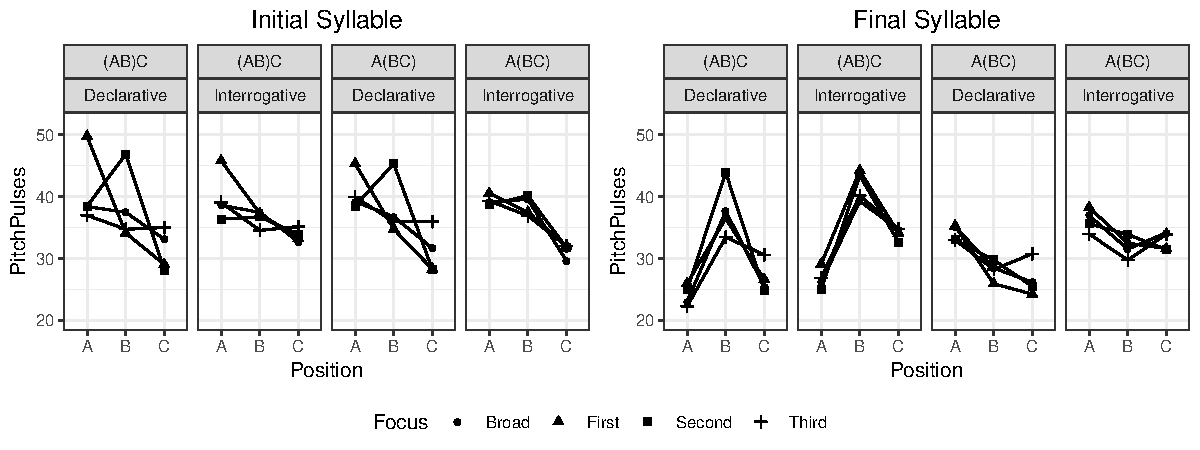
\includegraphics[width=5in]{Figures/PitchPulses.pdf}
		\caption{Number of pitch pulses of initial and final syllable for each target word}
		\label{figurePitchPulses}
	\end{center}
\end{figure*}


\begin{figure*}[htb!]
	\begin{center}
		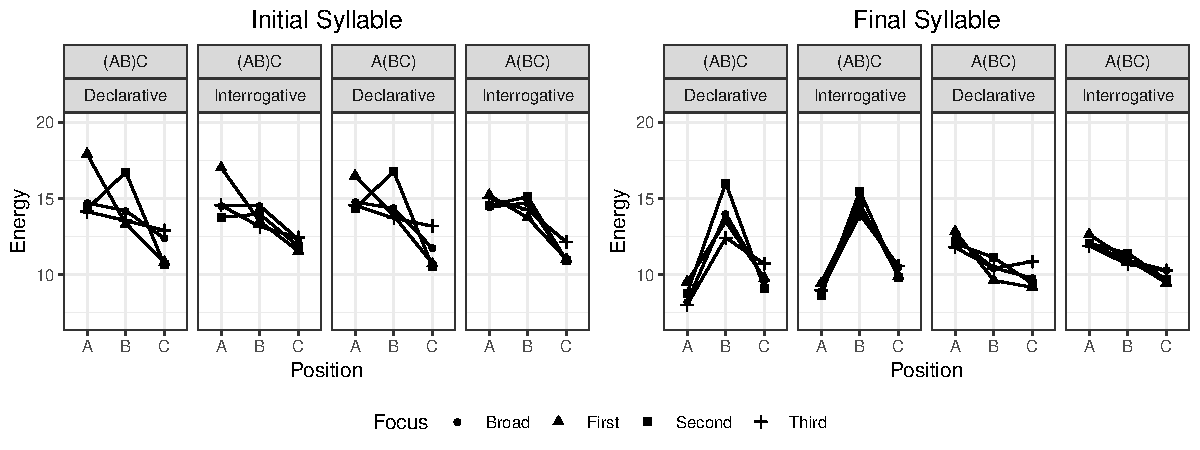
\includegraphics[width=5in]{Figures/Energy.pdf}
		\caption{Energy of initial and final syllable for each target word}
		\label{figureEnergy}
	\end{center}
\end{figure*}


\newpage
\subsection{Regression models for word A and word C}



\begin{table}[h!]
\begin{center}
\begin{footnotesize}
\begin{tabular}{l D{)}{)}{11)3} D{)}{)}{11)3} }
\hline
 & \multicolumn{1}{c}{Initial} & \multicolumn{1}{c}{Final} \\
\hline
(Intercept)                                 & 0.22 \; (0.02)^{***}  & 0.16 \; (0.02)^{**}  \\
Broad.vs.Narrow                             & 0.01 \; (0.01)        & 0.00 \; (0.00)       \\
First.vs.Late                               & -0.03 \; (0.01)^{***} & -0.01 \; (0.00)^{**} \\
Second.vs.Third                             & 0.00 \; (0.01)        & -0.00 \; (0.00)      \\
Decl.vs.Inter                               & 0.00 \; (0.00)        & 0.00 \; (0.00)       \\
Left.vs.Right                               & -0.00 \; (0.00)       & 0.05 \; (0.01)^{***} \\
Broad.vs.Narrow:Decl.vs.Inter               & -0.00 \; (0.01)       & -0.00 \; (0.01)      \\
First.vs.Late:Decl.vs.Inter                 & 0.01 \; (0.01)        & 0.01 \; (0.01)       \\
Second.vs.Third:Decl.vs.Inter               & 0.00 \; (0.01)        & 0.00 \; (0.01)       \\
Broad.vs.Narrow:Left.vs.Right               & -0.00 \; (0.01)       & -0.01 \; (0.01)      \\
First.vs.Late:Left.vs.Right                 & 0.03 \; (0.01)^{***}  & 0.00 \; (0.01)       \\
Second.vs.Third:Left.vs.Right               & -0.00 \; (0.01)       & 0.00 \; (0.01)       \\
Decl.vs.Inter:Left.vs.Right                 & 0.01 \; (0.01)        & -0.01 \; (0.01)      \\
Broad.vs.Narrow:Decl.vs.Inter:Left.vs.Right & 0.01 \; (0.01)        & 0.02 \; (0.01)       \\
First.vs.Late:Decl.vs.Inter:Left.vs.Right   & 0.00 \; (0.01)        & -0.00 \; (0.01)      \\
Second.vs.Third:Decl.vs.Inter:Left.vs.Right & -0.01 \; (0.02)       & -0.03 \; (0.02)^{*}  \\
\hline
\multicolumn{3}{l}{\tiny{$^{***}p<0.001$, $^{**}p<0.01$, $^*p<0.05$}}
\end{tabular}
\end{footnotesize}
\caption{Mixed Effects Regression Models for the duration of word A (estimate in ms, SE in parentheses).}
\label{modelDurationA}
\end{center}
\end{table}



\begin{table}[h!]
\begin{center}
\begin{footnotesize}
\begin{tabular}{l D{)}{)}{11)3} D{)}{)}{11)2} }
\hline
 & \multicolumn{1}{c}{Initial} & \multicolumn{1}{c}{Final} \\
\hline
(Intercept)                                 & 0.18 \; (0.03)^{**}   & 0.16 \; (0.03)^{**} \\
Broad.vs.Narrow                             & -0.00 \; (0.00)       & -0.00 \; (0.00)     \\
First.vs.Late                               & 0.01 \; (0.01)        & 0.01 \; (0.00)      \\
Second.vs.Third                             & 0.02 \; (0.01)^{*}    & 0.01 \; (0.01)      \\
Decl.vs.Inter                               & 0.00 \; (0.00)        & -0.00 \; (0.00)     \\
Left.vs.Right                               & -0.01 \; (0.00)       & -0.00 \; (0.00)     \\
Broad.vs.Narrow:Decl.vs.Inter               & 0.00 \; (0.00)        & -0.01 \; (0.00)^{*} \\
First.vs.Late:Decl.vs.Inter                 & -0.01 \; (0.00)       & 0.00 \; (0.00)      \\
Second.vs.Third:Decl.vs.Inter               & -0.02 \; (0.01)^{***} & -0.01 \; (0.01)^{*} \\
Broad.vs.Narrow:Left.vs.Right               & 0.01 \; (0.00)        & -0.01 \; (0.00)     \\
First.vs.Late:Left.vs.Right                 & 0.01 \; (0.00)        & 0.01 \; (0.00)^{*}  \\
Second.vs.Third:Left.vs.Right               & 0.00 \; (0.01)        & -0.01 \; (0.01)     \\
Decl.vs.Inter:Left.vs.Right                 & -0.01 \; (0.00)^{*}   & -0.00 \; (0.00)     \\
Broad.vs.Narrow:Decl.vs.Inter:Left.vs.Right & 0.00 \; (0.01)        & -0.00 \; (0.01)     \\
First.vs.Late:Decl.vs.Inter:Left.vs.Right   & 0.00 \; (0.01)        & -0.01 \; (0.01)     \\
Second.vs.Third:Decl.vs.Inter:Left.vs.Right & 0.00 \; (0.01)        & -0.01 \; (0.01)     \\
\hline
\multicolumn{3}{l}{\tiny{$^{***}p<0.001$, $^{**}p<0.01$, $^*p<0.05$}}
\end{tabular}
\end{footnotesize}
\caption{Mixed Effects Regression Models for the duration of word C (estimate in sec, SE in parentheses).}
\label{modelDurationC}
\end{center}
\end{table}



\begin{table}[h!]
\begin{center}
\begin{footnotesize}
\begin{tabular}{l D{)}{)}{11)3} D{)}{)}{11)3} }
\hline
 & \multicolumn{1}{c}{Initial} & \multicolumn{1}{c}{Final} \\
\hline
(Intercept)                                 & 62.54 \; (1.22)^{***} & 58.78 \; (1.04)^{***} \\
Broad.vs.Narrow                             & 0.13 \; (0.19)        & -0.55 \; (0.40)       \\
First.vs.Late                               & 0.10 \; (0.20)        & 0.53 \; (0.30)        \\
Second.vs.Third                             & 0.01 \; (0.19)        & 0.35 \; (0.26)        \\
Decl.vs.Inter                               & -0.44 \; (0.34)       & 0.64 \; (0.36)        \\
Left.vs.Right                               & 0.49 \; (0.21)        & -2.94 \; (0.78)^{*}   \\
Broad.vs.Narrow:Decl.vs.Inter               & -0.18 \; (0.31)       & -0.21 \; (0.42)       \\
First.vs.Late:Decl.vs.Inter                 & 0.69 \; (0.34)^{*}    & -1.10 \; (0.46)^{*}   \\
Second.vs.Third:Decl.vs.Inter               & -0.22 \; (0.39)       & -0.38 \; (0.52)       \\
Broad.vs.Narrow:Left.vs.Right               & -0.44 \; (0.31)       & 0.51 \; (0.42)        \\
First.vs.Late:Left.vs.Right                 & -0.76 \; (0.34)^{*}   & 0.12 \; (0.46)        \\
Second.vs.Third:Left.vs.Right               & -0.18 \; (0.38)       & -0.69 \; (0.52)       \\
Decl.vs.Inter:Left.vs.Right                 & -0.31 \; (0.27)       & 0.32 \; (0.37)        \\
Broad.vs.Narrow:Decl.vs.Inter:Left.vs.Right & -0.28 \; (0.62)       & -0.63 \; (0.84)       \\
First.vs.Late:Decl.vs.Inter:Left.vs.Right   & 0.59 \; (0.68)        & -0.42 \; (0.92)       \\
Second.vs.Third:Decl.vs.Inter:Left.vs.Right & 0.79 \; (0.77)        & 2.19 \; (1.05)^{*}    \\
\hline
\multicolumn{3}{l}{\tiny{$^{***}p<0.001$, $^{**}p<0.01$, $^*p<0.05$}}
\end{tabular}
\end{footnotesize}
\caption{Mixed Effects Regression Models for the mean intensity of word A (estimate in dB, SE in parentheses).}
\label{modelIntensityA}
\end{center}
\end{table}



\begin{table}[h!]
\begin{center}
\begin{footnotesize}
\begin{tabular}{l D{)}{)}{11)3} D{)}{)}{11)3} }
\hline
 & \multicolumn{1}{c}{Initial} & \multicolumn{1}{c}{Final} \\
\hline
(Intercept)                                 & 60.78 \; (1.30)^{***} & 57.72 \; (1.40)^{***} \\
Broad.vs.Narrow                             & -0.53 \; (0.19)       & -0.51 \; (0.31)       \\
First.vs.Late                               & 0.10 \; (0.21)        & 0.02 \; (0.19)        \\
Second.vs.Third                             & 1.07 \; (0.24)^{*}    & 0.68 \; (0.23)        \\
Decl.vs.Inter                               & 0.03 \; (0.29)        & 3.22 \; (0.48)^{***}  \\
Left.vs.Right                               & -0.36 \; (0.20)       & -0.00 \; (0.18)       \\
Broad.vs.Narrow:Decl.vs.Inter               & 1.24 \; (0.35)^{***}  & 1.04 \; (0.36)^{**}   \\
First.vs.Late:Decl.vs.Inter                 & -1.05 \; (0.38)^{**}  & -0.17 \; (0.39)       \\
Second.vs.Third:Decl.vs.Inter               & -1.76 \; (0.43)^{***} & -0.58 \; (0.44)       \\
Broad.vs.Narrow:Left.vs.Right               & 0.06 \; (0.35)        & 0.20 \; (0.36)        \\
First.vs.Late:Left.vs.Right                 & 0.32 \; (0.38)        & -0.46 \; (0.39)       \\
Second.vs.Third:Left.vs.Right               & 0.04 \; (0.43)        & -0.06 \; (0.44)       \\
Decl.vs.Inter:Left.vs.Right                 & 0.16 \; (0.30)        & -0.20 \; (0.31)       \\
Broad.vs.Narrow:Decl.vs.Inter:Left.vs.Right & -0.89 \; (0.69)       & -0.06 \; (0.71)       \\
First.vs.Late:Decl.vs.Inter:Left.vs.Right   & -0.63 \; (0.76)       & -0.09 \; (0.78)       \\
Second.vs.Third:Decl.vs.Inter:Left.vs.Right & -1.53 \; (0.86)       & 0.13 \; (0.88)        \\
\hline
\multicolumn{3}{l}{\tiny{$^{***}p<0.001$, $^{**}p<0.01$, $^*p<0.05$}}
\end{tabular}
\end{footnotesize}
\caption{Mixed Effects Regression Models for the mean intensity of word C (estimate in dB, SE in parentheses).}
\label{modelIntensityC}
\end{center}
\end{table}



\begin{table}[h!]
\begin{center}
\begin{footnotesize}
\begin{tabular}{l D{)}{)}{12)3} D{)}{)}{12)3} }
\hline
 & \multicolumn{1}{c}{Initial} & \multicolumn{1}{c}{Final} \\
\hline
(Intercept)                                 & 199.66 \; (8.23)^{***} & 197.04 \; (9.02)^{***} \\
Broad.vs.Narrow                             & 2.55 \; (3.00)         & -4.00 \; (1.85)^{*}    \\
First.vs.Late                               & -12.99 \; (5.01)^{*}   & -5.24 \; (2.74)        \\
Second.vs.Third                             & 3.40 \; (1.79)         & 3.69 \; (2.08)         \\
Decl.vs.Inter                               & -5.16 \; (2.79)        & 12.98 \; (3.71)^{**}   \\
Left.vs.Right                               & 2.68 \; (2.34)         & 3.17 \; (2.66)         \\
Broad.vs.Narrow:Decl.vs.Inter               & -5.18 \; (2.88)        & 0.43 \; (3.37)         \\
First.vs.Late:Decl.vs.Inter                 & 8.87 \; (3.17)^{**}    & -10.72 \; (3.69)^{**}  \\
Second.vs.Third:Decl.vs.Inter               & -0.83 \; (3.59)        & 4.21 \; (4.16)         \\
Broad.vs.Narrow:Left.vs.Right               & -0.21 \; (2.89)        & -3.14 \; (3.37)        \\
First.vs.Late:Left.vs.Right                 & 2.78 \; (3.17)         & -6.23 \; (3.69)        \\
Second.vs.Third:Left.vs.Right               & 0.11 \; (3.57)         & -3.67 \; (4.16)        \\
Decl.vs.Inter:Left.vs.Right                 & -0.24 \; (2.55)        & 0.82 \; (2.97)         \\
Broad.vs.Narrow:Decl.vs.Inter:Left.vs.Right & 1.85 \; (5.77)         & -3.96 \; (6.73)        \\
First.vs.Late:Decl.vs.Inter:Left.vs.Right   & -3.25 \; (6.34)        & 1.54 \; (7.38)         \\
Second.vs.Third:Decl.vs.Inter:Left.vs.Right & -7.04 \; (7.18)        & -7.62 \; (8.33)        \\
\hline
\multicolumn{3}{l}{\tiny{$^{***}p<0.001$, $^{**}p<0.01$, $^*p<0.05$}}
\end{tabular}
\end{footnotesize}
\caption{Mixed Effects Regression Models for the Max F$_0$ of word A (estimate in Hz, SE in parentheses).}
\label{modelPitchA}
\end{center}
\end{table}



\begin{table}[h!]
\begin{center}
\begin{footnotesize}
\begin{tabular}{l D{)}{)}{12)3} D{)}{)}{12)3} }
\hline
 & \multicolumn{1}{c}{Initial} & \multicolumn{1}{c}{Final} \\
\hline
(Intercept)                                 & 190.54 \; (7.65)^{***} & 197.40 \; (8.84)^{***} \\
Broad.vs.Narrow                             & 0.10 \; (3.69)         & 1.50 \; (2.63)         \\
First.vs.Late                               & 2.31 \; (3.67)^{**}    & 1.75 \; (2.37)         \\
Second.vs.Third                             & 10.43 \; (6.27)^{***}  & 13.26 \; (4.71)        \\
Decl.vs.Inter                               & 3.30 \; (2.84)         & 47.31 \; (7.35)^{*}    \\
Left.vs.Right                               & -1.43 \; (1.90)        & -0.73 \; (2.46)        \\
Broad.vs.Narrow:Decl.vs.Inter               & 14.56 \; (3.98)        & 6.20 \; (4.32)^{**}    \\
First.vs.Late:Decl.vs.Inter                 & -14.50 \; (4.32)^{***} & -4.43 \; (4.73)^{***}  \\
Second.vs.Third:Decl.vs.Inter               & -26.74 \; (4.98)^{***} & -10.64 \; (5.44)       \\
Broad.vs.Narrow:Left.vs.Right               & 1.86 \; (3.97)         & 0.08 \; (4.30)         \\
First.vs.Late:Left.vs.Right                 & 3.01 \; (4.34)         & 7.57 \; (4.75)         \\
Second.vs.Third:Left.vs.Right               & -4.66 \; (4.95)        & -3.07 \; (5.39)        \\
Decl.vs.Inter:Left.vs.Right                 & -0.37 \; (3.50)^{*}    & -5.94 \; (3.82)        \\
Broad.vs.Narrow:Decl.vs.Inter:Left.vs.Right & -9.11 \; (7.92)        & -6.26 \; (8.60)        \\
First.vs.Late:Decl.vs.Inter:Left.vs.Right   & -2.66 \; (8.67)        & 8.21 \; (9.49)         \\
Second.vs.Third:Decl.vs.Inter:Left.vs.Right & -7.22 \; (9.90)^{*}    & 16.87 \; (10.80)       \\
\hline
\multicolumn{3}{l}{\tiny{$^{***}p<0.001$, $^{**}p<0.01$, $^*p<0.05$}}
\end{tabular}
\end{footnotesize}
\caption{Mixed Effects Regression Models for the mean F$_0$ of word C (estimate in Hz, SE in parentheses).}
\label{modelPitchC}
\end{center}
\end{table}


\newpage


\begin{figure*}[ht!]
	\begin{center}
	{\footnotesize
		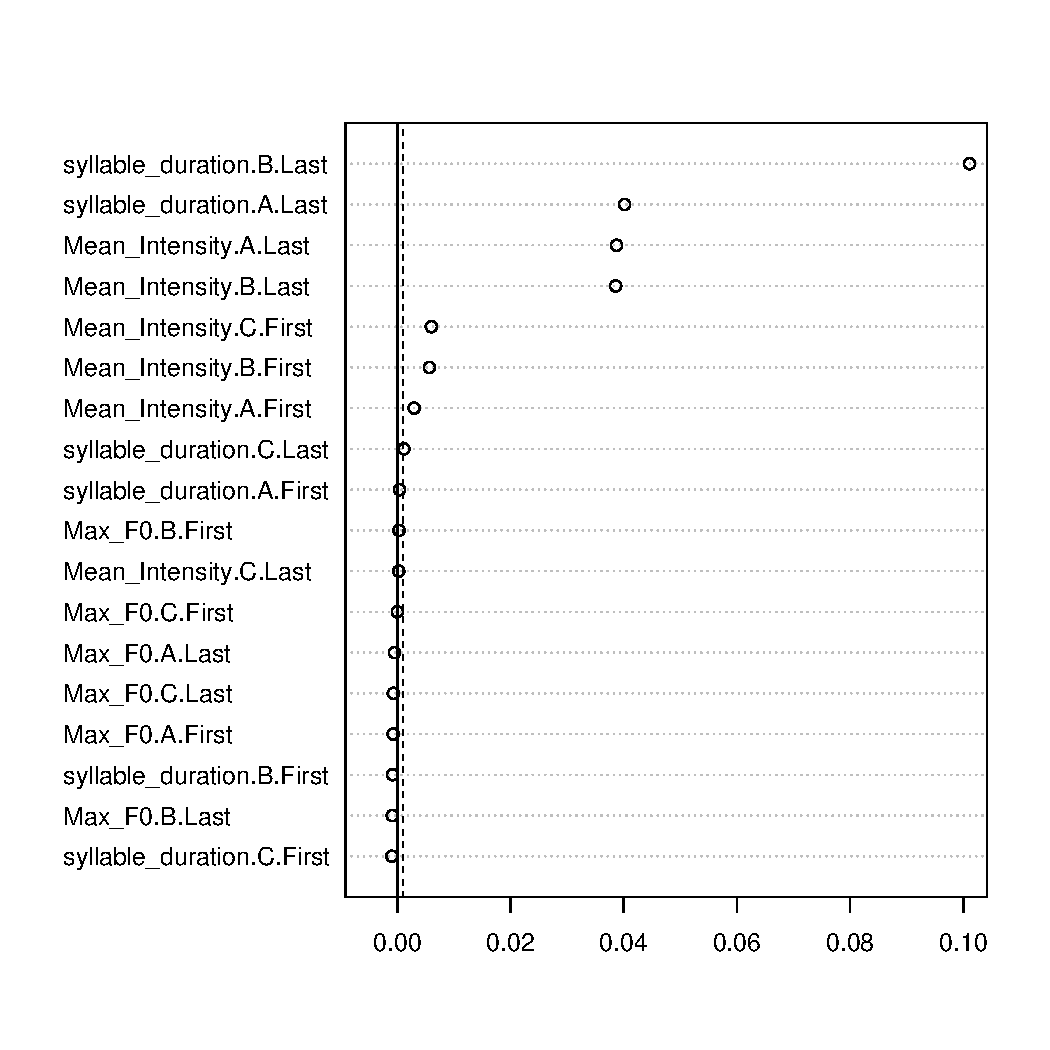
\includegraphics[width=2.8in]{Figures/phrasingFirstCVarimp.pdf}	
		}
		\caption{Importance of variables in random forest classification of Constituency for the case of broad focus (left) and first focus (right) respectively}
		\label{focusForestFirstC}
	\end{center}
\end{figure*}




\end{document}

